\documentclass[11pt]{report}
\usepackage[a4paper]{geometry}
\usepackage{outline}
\usepackage{pmgraph}
\usepackage[normalem]{ulem}
\usepackage{graphicx}
\usepackage{booktabs}
\usepackage{amsmath}
\usepackage{amsthm}
\usepackage{eucal}
\usepackage{amssymb}
\usepackage{mathrsfs}
\usepackage{tikz}
\usepackage{pgf}
\usepackage{lscape}
\usetikzlibrary{arrows,automata}
\usepackage{verbatim}
\usepackage{float}
\usepackage{appendix}
\allowdisplaybreaks
\usepackage{listings}
\usepackage{multirow}
\usepackage{url}
\usepackage{color}
\usepackage{nicefrac}
\usepackage[intoc]{nomencl}
\lstset{language=matlab,frame=single}
\usepackage[framed,numbered,autolinebreaks,useliterate]{mcode}
\setcounter{secnumdepth}{5}
\setcounter{tocdepth}{4}
\usepackage{tocloft}
\usepackage{blkarray}
\usepackage{placeins}
\usepackage{tkz-berge}
\thispagestyle{empty}
\usetikzlibrary{fit,shapes}

\makenomenclature
\renewcommand{\nomname}{List of Symbols and Abbreviations}

\usepackage{ifthen}
  \renewcommand{\nomgroup}[1]{%
  \item[\bfseries
  \ifthenelse{\equal{#1}{A}}{Abbreviations}{%
  \ifthenelse{\equal{#1}{B}}{PageRank Notation}{%
  \ifthenelse{\equal{#1}{C}}{HITS Notation}{%
  \ifthenelse{\equal{#1}{D}}{SALSA Notation}{}}}}%
  ]}

\title{\textbf{PageRank and Random Walks on the Web}}
\author{Shannon Chatha}
\date{\today}

\begin{document}

%--------------------Title Page
\maketitle
\begin{abstract}
This project...
\end{abstract}
\newpage
\vspace*{\fill}
\begin{center}
\textbf{Declaration of Authorship}\\ 
\textit{This piece of work is a result of my own work except where it forms an assessment
based on group project work. In the case of a group project, the work
has been prepared in collaboration with other members of the group. Material
from the work of others not involved in the project has been acknowledged and
quotations and paraphrases suitably indicated.}
\end{center}
\vspace*{\fill}
\mbox{}
\nomenclature[01]{$r(P_i)$}{Rank of page \textit{i}}
\nomenclature[02]{$\boldsymbol{\pi}$}{PageRank vector}
 
\nomenclature[A,01]{PR}{PageRank}
\nomenclature[A,02]{HITS}{Hypertext Induced Topic Search}
\nomenclature[A,03]{SALSA}{Stochastic Approach to Linear Systems Analysis}
\nomenclature[A,04]{TKC}{Tightly Knitted Community}
\nomenclature[A,05]{WPR}{Weighted PageRank}
\nomenclature[A,06]{TSPR}{Topic-Specific PageRank}

\nomenclature[B,01]{\textbf{H}}{Hyperlink Matrix}
\nomenclature[B,02]{\textbf{S}}{Stochastic Matrix}
\nomenclature[B,03]{$1^T$}{Rank 1 matrix with unit entries of size $[1 \times n]$}
\nomenclature[B,04]{\textbf{a}}{Dangling node vector}
\nomenclature[B,05]{\textbf{G}}{Google Matrix}
\nomenclature[B,06]{$\alpha$}{Scaling parameter $\in$ [0,1]}
\nomenclature[B,07]{$\textbf{v}^T$}{Personalization vector}

\nomenclature[C,01]{N}{Neighbourhood graph}
\nomenclature[C,02]{\textbf{L}}{Adjacency Matrix}
\nomenclature[C,03]{\textbf{e}}{Rank 1 matrix with unit entries of size $[1 \times n]$}
\nomenclature[C,04]{$\textbf{L}^T\textbf{L}$}{Authority Matrix}
\nomenclature[C,05]{$\textbf{LL}^T$}{Hub Matrix}
\nomenclature[C,06]{\textbf{x}}{Authority vector}
\nomenclature[C,07]{\textbf{y}}{Hub vector}

\nomenclature[D,01]{N}{Neighbourhood graph}
\nomenclature[D,02]{G}{Bipartite undirected graph}
\nomenclature[D,03]{$\textbf{L}_r$}{\textbf{L} with each non-zero row divided by row sum}
\nomenclature[D,04]{$\textbf{L}_c$}{\textbf{L} with each non-zero column divided by column sum}
\nomenclature[D,05]{\textbf{A}}{Authority Matrix}
\nomenclature[D,06]{\textbf{H}}{Hub Matrix}
\nomenclature[D,08]{$\boldsymbol{\pi}_h^T$}{Hub vector}
\nomenclature[D,07]{$\boldsymbol{\pi}_a^T$}{Authority vector}

\tableofcontents
\newpage
\listoffigures
\listoftables

\addcontentsline{toc}{chapter}{List of Figures}
\addcontentsline{toc}{chapter}{List of Tables}


\printnomenclature[5em]

 



%--------------------Introduction

\chapter{Introduction}\label{chap:intro}
Google's PageRank algorithm, developed in 1998 by Sergey Brin and Larry Page is one of the most well-known and influential methods of ranking web pages. The hyperlink structure of the web is represented by a directed graph, with the web pages representing the nodes and the links between nodes being the hyperlinks. Inlinks are pages that point into nodes, and outlinks point out from nodes \cite{brin1998anatomy}. The algorithm in its simplest form aims to rank pages with the assumption that a web page's importance is reliant on other important pages linking to it. When this is represented mathematically, it becomes clear that the importance scores of the web pages relate to the stationary points of a Markov chain, and hence Markov theory and matrices can be used to solve the PageRank equation:
\begin{equation}
\boldsymbol{\pi} = \boldsymbol{\pi} \cdot \textbf{G}
\end{equation}
where \textbf{G} is the 'Google Matrix' and $\boldsymbol{\pi}$ is the set of ranked web pages \cite{langville}. We are able to interpret a web pages PageRank as the fraction of time that a random surfer spends on that web page, with the random surfer more likely to return to the most important pages \cite{bonato}. Throughout this report we will be using the network graph as an example: 
\begin{figure}[H]
\centering
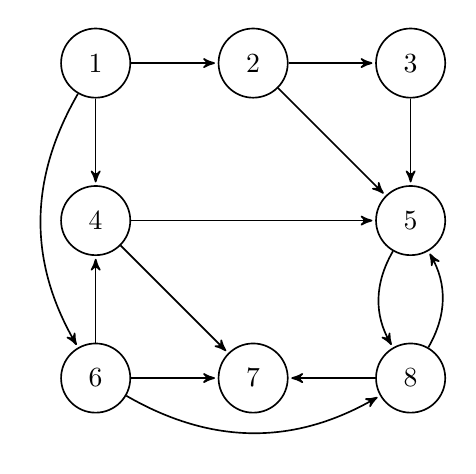
\begin{tikzpicture}[->,>=stealth',shorten >=1pt,auto,node distance=2cm,
                    semithick]
\tikzstyle{every state}=[fill=white,draw=black,text=black]
\node[state] (1) {$1$};
\node[state] (2) [right of=1] {$2$};
\node[state] (3) [right of=2] {$3$};
\node[state] (4) [below of=1] {$4$};
\node[state] (5) [below of=3] {$5$};
\node[state] (6) [below of=4] {$6$};
\node[state] (7) [right of=6] {$7$};
\node[state] (8) [right of=7] {$8$};
\path (1) edge node{} (2)
          edge node{} (4)
          edge [bend right] node{} (6)
      (2) edge node{} (3)
          edge node{} (5)
      (3) edge node{} (5)
      (4) edge node{} (7)
          edge node{} (5)
      (5) edge [bend right] node{} (8)
      (6) edge node{} (4)
          edge node{} (7)
          edge [bend right] node{} (8)
      (8) edge [bend right] node{} (5)
          edge node{} (7);
          
\end{tikzpicture}
\caption{Graph modelling 8-node web} \label{fig:Example}
\end{figure}

In the first chapter of this report, we will explore mathematical representations of the PageRank equation, the modifications required on the matrix in order to use Markov theory to solve the PageRank equation, and finally on the use of the power method to solve the equation. Chapter \ref{chap:Other} discusses other methods of ranking web pages, and compares these to PageRank. Chapter \ref{chap:Improve} will then explore improvements to the PageRank representation that could increase the accuracy and personalise the PageRank method for a user, such as weighted PageRank and topic-specific PageRank. Chapter \ref{chap:Applications} explores potential applications for PageRank beyond ranking web-pages, for example in predicting traffic flow in Durham. The final chapter of the report, Chapter \ref{chap:Conclusion}, summarises the main points of the report.



%--------------------Matrix Representation 
\chapter{Mathematical Representation} \label{chap:Math}
In this chapter we aim to represent the PageRank equation mathematically, in Section \ref{sec:summ}, we use summation formulas to represent the algorithm, and introduce the idea of an iterative process to compute the PageRank vector. In Section \ref{sec:matrix} we represent the PageRank equation using matrices, and discuss the two adjustments required in order to use Markov theory to solve the PageRank equation leading to the formation of a dense Google Matrix. We will discuss the use of the power method to solve the PageRank equation in Section \ref{sec:solve}.

The references Austin \cite{austin}, Bonato \cite{bonato} and Langville \cite{langville} were consulted during the writing of this chapter, and the material has been collated below.  

\section{Summation Formula of PageRank} \label{sec:summ}
In order to mathematically represent the PageRank algorithm, Brin and Page first assigned each page, $P_i$, a rank
\begin{equation}
r(P_i) = \displaystyle \sum_{P_j\in B_{P_i }} \frac{r(P_j)}{|P_j|}
\end{equation} where $B_{P_i}$ is the set of pages pointing into $P_i$, and $\vert P_j\vert$ is the number of outlinks from a page. However the ranking of outlinks is unknown, and so an iterative summation formula is required, where it is assumed that all pages have equal PageRank at the start, \(r_o = \frac{1}{n}\) , \begin{equation} \label{eq:iterative}
r_{(k+1)}P_i = \displaystyle \sum_{P_j\in B_{P_i }}\frac{r_k(P_j)}{|P_j|}
\end{equation} 
When Equation \eqref{eq:iterative} is applied to all pages in the graph, you can calculate a ranking for the pages, so for the graph in Figure \ref{fig:Example}, we get the following values for the PageRanks after some iterations: 

\begin{table}[H] \caption{First iterates using Equation \eqref{eq:iterative} on Figure \ref{fig:Example}}
 \centering
 \begin{tabular} {c c c |c} 
 Iter. 0 & Iter. 1 & Iter. 2 &  Rank at Iter. 2 \\ [0.5ex] 
 \hline
 $r_0(P_1)=\frac{1}{8}$ & $r_1(P_1)=0$ & $r_2(P_1)=0$ & $6$ \\ 
 $r_0(P_2)=\frac{1}{8}$ & $r_1(P_2)=\frac{1}{24}$ & $r_2(P_2)=0$ & $6$ \\ 
 $r_0(P_3)=\frac{1}{8}$ & $r_1(P_3)=\frac{1}{16}$ & $r_2(P_3)=\frac{1}{48}$ & $4$ \\ 
 $r_0(P_4)=\frac{1}{8}$ & $r_1(P_4)=\frac{5}{48}$ & $r_2(P_4)=\frac{1}{48}$ & $4$ \\ 
 $r_0(P_5)=\frac{1}{8}$ & $r_1(P_5)=\frac{5}{16}$ & $r_2(P_5)=\frac{11}{48}$ & $2$ \\ 
 $r_0(P_6)=\frac{1}{8}$ & $r_1(P_6)=\frac{1}{24}$ & $r_2(P_6)=0$ & $6$ \\ 
 $r_0(P_7)=\frac{1}{8}$ & $r_1(P_7)=\frac{3}{16}$ & $r_2(P_7)=\frac{1}{6}$ & $3$ \\ 
 $r_0(P_8)=\frac{1}{8}$ & $r_1(P_8)=\frac{3}{16}$ & $r_2(P_8)=\frac{1}{3}$ & $1$ \\ \end{tabular}
\label{Table:Summ}
\end{table}

\section{Matrix Representation} \label{sec:matrix}
\subsection{Hyperlink Matrix} \label{sec:hyperlink}
If we represent the PageRank algorithm using matrices, we are able to compute a $ [1 \times \textit{n}]$ row vector, $\boldsymbol{\pi}^T$, the PageRank vector, at each iteration which contains the PageRank values for all web pages in the hyperlink graph. In order to do this we first introduce the concept of the Hyperlink matrix, a $[\textit{n}\times \textit{n}]$ matrix \textbf{H}, which is a row normalized matrix where 
\(\boldsymbol{H_{ij}} = \begin{cases} \frac{1}{\vert P_j \vert} & P_j\in B_{P_i } \\ 0 & \textnormal{otherwise} \end{cases}\). So for Figure \ref{fig:Example} we are able to produce 
\[\textbf{H}=\left(
\begin{array}{cccccccc}
0 & \frac{1}{3} & 0 & \frac{1}{3} & 0 &\frac{1}{3} & 0& 0 \\
0 & 0 &\frac{1}{2}& 0 &\frac{1}{2}& 0 & 0 & 0\\
0 & 0 & 0 & 0 & 1 & 0 & 0 & 0\\
0 & 0 & 0 & 0 & \frac{1}{2} & 0 & \frac{1}{2} & 0\\
0 & 0 & 0 & 0 & 0 & 0 & 0 & 1\\
0 & 0 & 0 & \frac{1}{3} & 0 & 0 & \frac{1}{3} & \frac{1}{3} \\
0 & 0 & 0 & 0 & 0 & 0 & 0 & 0\\
0 & 0 & 0 & 0 & \frac{1}{2} & 0 & \frac{1}{2} & 0\\
\end{array}
\right)	\]

The non-zero elements of row \textit{i} relate to the outlinking pages of $P_i$, for example, node 1 has outlinks to pages 2, 4 and 6, and so in columns 2, 4 and 6 of \textbf{H} the value in row 1 are $\frac{1}{3}$ and the non-zero elements of column \textit{i} relates to the inlinking pages.

We are able to write Equation \eqref{eq:iterative} as \begin{equation} \label{eq:power H}
\boldsymbol\pi^{(k+1)T} = \boldsymbol\pi^{(k)T}\textbf{H}
\end{equation}  which shows that the vector $\boldsymbol\pi^T$ is an eigenvector of the matrix \textbf{H} with eigenvalue 1, otherwise known as the stationary vector of \textbf{H}, essentially this is the classical power method applied to \textbf{H}. We are able to observe that \textbf{H} is a very sparse matrix, as the majority of its entries are 0, which is computationally very beneficial, as it reduces the vector-matrix multiplication at each iteration to a linear computation. The formation of \textbf{H} is very similar to the formation of a transition probability matrix for a Markov chain, and it is also noted that \textbf{H} is similar to a stochastic matrix, as all entries are non-negative, however not all rows sum to 1.

From Markov theory, we know that for any starting vector, the power method applied to a matrix, \textbf{M},  will converge to a stationary vector as long as \textbf{M} is stochastic, irreducible and aperiodic. However, \textbf{H} is not guaranteed to converge due to the presence of rank sinks. A rank sink is a page that stores PageRank with each iteration, this can be in the form of dangling nodes, which are nodes that have no outlinks, for example 
\begin{figure}[h]
\centering
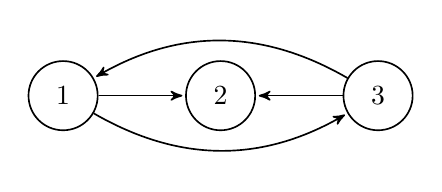
\begin{tikzpicture}[->,>=stealth',shorten >=1pt,auto,node distance=2cm,
                    semithick]
\tikzstyle{every state}=[fill=white,draw=black,text=black]
\node[state] (1) {$1$};
\node[state] (2) [right of=1] {$2$};
\node[state] (3) [right of=2] {$3$};
\path (1) edge node{} (2)
          edge [bend right] node{} (3)
      (3) edge [bend right] node{} (1)
          edge node{} (2);
\end{tikzpicture} \caption{Simple graph with rank sink} \label{fig:dangling} 
\end{figure} in Figure \ref{fig:dangling}, node 2 is a dangling node. There can also be an issue with cycles,
\begin{figure}[h]
\centering
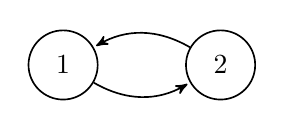
\begin{tikzpicture}[->,>=stealth',shorten >=1pt,auto,node distance=2cm,
                    semithick]
\tikzstyle{every state}=[fill=white,draw=black,text=black]
\node[state] (1) {$1$};
\node[state] (2) [right of=1] {$2$};
\path (1) edge [bend right] node{} (2)
      (2) edge [bend right] node{} (1);
\end{tikzpicture} \caption{Simple graph with cycle} \label{fig:cycle}
\end{figure} for example in Figure \ref{fig:cycle}, an infinite loop is created between nodes 1 and 2, and so the iterate will not converge. We are able to apply modifications to \textbf{H} which make it a Markov matrix.

\subsection{Stochastic Matrix} \label{sec:stoc}
The first modification, called the stochasticity adjustment, leads to the formation of a stochastic matrix, \textbf{S}. In the stochasticity adjustment, we change rows of 0's to rows of $\frac{1}{n}$, hence making \textbf{S} stochastic, as all rows now sum to 1. Mathematically this is shown as, \begin{equation} \label{eq:s}
\textbf{S} = \textbf{H} + \textbf{a}\left(\frac{1}{n}\cdot 1^{T}\right)
\end{equation} 
where \textbf{a} is the dangling node vector, \(\boldsymbol{a} = \begin{cases} 1 & \textnormal{if dangling node} \\ 0 & \textnormal{otherwise} \end{cases}\), and $1^T$ is the rank 1 matrix with unit entries of size $[1\times n]$.

In terms of the random surfer idea as mentioned in section 1.1, this means that if the surfer enters a dangling node, it is able to teleport to another page in the graph at random. For the 8-node graph example in Figure \ref{fig:Example}, we produce  
\[ \renewcommand*{\arraystretch}{1.25} \textbf{S}=\left(
\begin{array}{cccccccc}
0 & \frac{1}{3} & 0 & \frac{1}{3} & 0 &\frac{1}{3} & 0& 0 \\
0 & 0 &\frac{1}{2}& 0 &\frac{1}{2}& 0 & 0 & 0\\
0 & 0 & 0 & 0 & 1 & 0 & 0 & 0\\
0 & 0 & 0 & 0 & \frac{1}{2} & 0 & \frac{1}{2} & 0\\
0 & 0 & 0 & 0 & 0 & 0 & 0 & 1\\
0 & 0 & 0 & \frac{1}{3} & 0 & 0 & \frac{1}{3} & \frac{1}{3} \\
\frac{1}{8} & \frac{1}{8} & \frac{1}{8} & \frac{1}{8} & \frac{1}{8} & \frac{1}{8} & \frac{1}{8} & \frac{1}{8}\\
0 & 0 & 0 & 0 & \frac{1}{2} & 0 & \frac{1}{2} & 0\\
\end{array}
\right)	\] This modification ensures that \textbf{S} is stochastic, but not that it is irreducible and aperiodic and so it is not guaranteed that it will converge when using the power method.

The stochasticity adjustment is especially crucial when modelling the web in practice, as in an analysis of a significant section of the web graph, only a quarter of the web is strongly connected, and so a large majority of the web are dangling nodes \cite{chakrabarti2002mining}.

\subsection{Google Matrix}\label{sec:google}
The primitivity adjustment is the next modification to the matrix which ensures that it is both aperiodic and irreducible. This modification introduces a scaling parameter $\alpha \in [0,1]$. In terms of the random surfer, this adjustment means that most of the time the surfer will follow links from page $P_i$ to $P_j$, however at any time the surfer could choose a page uniformly at random from the graph and jump there. This adjustment is shown by 
\begin{equation}\label{eq:G}
\textbf{G}=\alpha\textbf{S}+\left((1-\alpha)\cdot\frac{1}{n}\cdot1^T\right)
\end{equation} 
where \textbf{G} is the Google matrix. For Figure \ref{fig:Example},
\[\textbf{G}=\alpha\textbf{S}+\left((1-\alpha)\cdot \frac{1}{8} \cdot \left(  \begin{array}{cccccccc}
1&1&1&1&1&1&1&1\end{array}\right) \right)\]

Due to the primitivity adjustment, \textbf{G} is stochastic, as it is the combination of two stochastic matrices, irreducible and aperiodic. This implies that the power method applied to \textbf{G} is guaranteed to converge to a stationary vector $\boldsymbol{\pi}^T$.
\begin{equation}\label{eq:power to G}
\boldsymbol{\pi}^{(k+1)T} = \boldsymbol{\pi}^{(k)T}\textbf{G}
\end{equation} 

However, \textbf{G} is artificial, as it has been modified twice in order to assure convergence, also \textbf{G} is dense, which is a computational disadvantage, this can be solved by expressing \textbf{G} in terms of \textbf{H}, a very sparse matrix; 
 
\begin{align}
\textbf{G} & = \alpha\textbf{S}+\left((1-\alpha)\cdot\frac{1}{n}\cdot1^T\right)\notag\\
& = \alpha \left(\textbf{H} + \textbf{a}\left(\frac{1}{n}\cdot 1^{T}\right)\right) + \left((1-\alpha)\cdot\frac{1}{n}\cdot1^T\right)\notag\\
& = \alpha\textbf{H} + (\alpha\textbf{a} +(1-\alpha))\left(\frac{1}{n}\cdot 1^T\right)\label{eq:G in H}
\end{align} 

\subsection{$\alpha$ parameter} \label{sec:alpha}
The $\alpha$ parameter introduced in the primitivity adjustment controls how much the original hyperlink structure of the web is weighted. As $\alpha \rightarrow 1$ the expected number of iterations required before convergence increases as the PageRank vector is more volatile, however artificiality is low, and we are close to working with the original hyperlink graph. When $\alpha =0$ then $\textbf{G}=\frac{1}{n}\cdot 1^T$, so there is a link between every page, and so the hyperlink structure has completely disappeared. 

Brin and Page suggested the value of 0.85, as this strikes a balance between efficiency and effectiveness. Using Figure \ref{fig:Example} and Equation \eqref{eq:G in H}, we obtain
\begin{equation}
\textbf{G} = \left(
\begin{array}{cccccccc}
0.019 & 0.302 & 0.019 & 0.302 & 0.019 & 0.302 & 0.019 & 0.019  \\
0.019 & 0.019 & 0.444 & 0.019 & 0.444 & 0.019 & 0.019 & 0.019  \\
0.019 & 0.019 & 0.019 & 0.019 & 0.869 & 0.019 & 0.019 & 0.019  \\
0.019 & 0.019 & 0.019 & 0.019 & 0.444 & 0.019 & 0.444 & 0.019  \\
0.019 & 0.019 & 0.019 & 0.019 & 0.019 & 0.019 & 0.019 & 0.869  \\
0.019 & 0.019 & 0.019 & 0.302 & 0.019 & 0.019 & 0.302 & 0.302  \\
0.125 & 0.125 & 0.125 & 0.125 & 0.125 & 0.125 & 0.125 & 0.125  \\
0.019 & 0.019 & 0.019 & 0.019 & 0.444 & 0.019 & 0.444 & 0.019 
\end{array}
\right)
\end{equation}
\section{Solving the PageRank Equation} \label{sec:solve}
In order to solve the PageRank equation we either need to solve the eigenvector problem for $\boldsymbol{\pi}^T$, \(\boldsymbol{\pi}^T = \boldsymbol{\pi}^T\textbf{G}\), i.e. we need to find a normalized dominant left-hand eigenvector of \textbf{G} which corresponds to the dominant eigenvalue of $\lambda_1 = 1$. We are also able to solve the equation by using a linear system \(\boldsymbol{\pi}^T(\textbf{I}-\textbf{G})=\textbf{0}^T\), where we want to find a normalized left-hand vector of \textbf{I}-\textbf{G}, \cite{langville}. We will discuss the power method in more detail in this report, as this is the original method proposed to solve the PageRank equation \cite{langville}.

\subsection{Power Method} \label{sec:power}
PERRON-FROBENIUS \cite{meyer2000matrix}  \cite{gallager1992discrete} 
\textcolor{red}{\textbf{EXPLAIN MATHS MORE HERE}} Perron-Frobenius theorem that a positive, stochastic, irreducible matrix is guaranteed to have a positive eigenvector \cite{thorson2004modeling}.

Using Matlab code as given in Appendix \ref{app:code}, 

\[\boldsymbol\pi = \left(
\begin{array}{c}
0.040 \\
0.051 \\
0.062 \\
0.066 \\
0.258 \\
0.051 \\
0.199 \\
0.274
\end{array}
\right)\]

\begin{table}[H] \caption{Ranking of web pages after two iterations and after the power method}
 \centering
 \begin{tabular} {c| c c} 
 Node & Rank at Iter. 2 & PR \\ [0.5ex] 
 \hline
 1&6&8\\
 2&6&6\\
 3&4&5\\
 4&4&4\\
 5&2&2\\
 6&6&6\\
 7&3&3\\
 8&1&1\\
 \end{tabular}
 \label{Table:PR and summ}
\end{table}

\subsection{Why the Power Method}\label{sec:why power}

The power method is useful for solving the PageRank equation as it converges to a unique vector, the PageRank vector, where the $i^{th}$ entry of $\boldsymbol\pi$ relates to the PageRank of \textit{i} \cite{ipsen2005analysis}. The main disadvantage of the power method is that it known to be very slow to converge, with the computation of the PageRank vector taking a few days to complete for the large web graph, but the power method is very simple. As we are able to simplify \textbf{G} to \textbf{H} as shown in Equation \eqref{eq:G in H}, the power method is very storage friendly, this is as for an iteration only a sparse \textbf{H}, a dangling node vector \textbf{a} and the current iterate are required to be stored \cite{langville}. Brin and Page reported that the PageRank vector converges to 2-3 degrees of accuracy within 50-100 iterations \cite{austin}. Pages with lower PR are converge very quickly when compared to pages with higher PR \cite{thorson2004modeling}.


%--------------------Comparison to other methods of Ranking web pages
\chapter{Other Methods of Ranking Web Pages}\label{chap:Other}


Whilst PR is the most influential algorithm for ranking web pages, there are many other algorithms that are well known and in some cases preferable. In this chapter we will discuss two such algorithms, Section \ref{sec:HITS} will discuss the HITS algorithm which also ranks web pages by popularity \cite{kleinberg1999authoritative}, however it differs to PR by producing two scores for each web page. HITS has been used in the search engine Ask.com \cite{bonato}, and expands upon the idea of using connectivity analysis to identify high quality pages within a topic specific graph \cite{manning}. We will also discuss the SALSA algorithm in Section \ref{sec:SALSA}, which incorporates ideas from both HITS and PR, as it assigns two scores to each web pages, but uses Markov theory to calculate these scores as in PR \cite{lempel2000stochastic}. We will discuss the strengths and weaknesses of these two algorithms, and compare these algorithms to PR in Section \ref{sec:compare}.

\section{HITS Algorithm} \label{sec:HITS}
The Hypertext Induced Topic Search (HITS) algorithm was developed by Jon Kleinburg, and is similar to PR as it ranks web pages by popularity, however HITS produces two popularity scores, for each web page.  Kleinburg developed this algorithm as a connectivity analysis on the hyper linked environment of the web. The algorithm manages to distil a broad topic down to a representation of a very small size \cite{kleinberg1999authoritative}. 

The HITS algorithm defines an authoritative page as a page with sources of information on a topic, while a hub is a page that is not in itself a source of information, but compilations to authoritative pages \cite{manning}. Authoritative pages have many inlinks, whilst a hub has many outlinks, each web page on a graph has some measure of an authority and some measure of a hub. A good authority is one which is pointed to by good hubs, whilst a good hub is one which points to good authorities. This cyclic definition is similar to the definition for PR, and we use an iterative computation in order to rank the web pages in the same manner.

The authority weight of a page is the sum of the hubness weights of its parents, which are the backlinks of a node, whilst the hubness weight of a page is the sum of the authority weights of its children, the forward links from a node \cite{baldi2003modeling}.

{Authorities are pages with good coverage of a topic, hubs are pages with links to many useful pages on a topic \cite{bonato}.} 

HITS was developed as a way to combat two problems that can occur when ranking web pages. One of these is the scarcity problem, where not many pages contain the exact information that you desire, and it can be difficult to identify the web pages that the user requires. The second problem that can occur is the abundance problem, where the number of pages that are returned to the user as being relevant to the query is too much for the human user to digest. 



\subsection{HITS Implementation} \label{sec:HITS implementation}
The HITS algorithm consists of two steps, the first step involves building a neighbourhood graph, N, which is related to the query term, and is known as the sampling step. The second step, the weight-propagation step, involves the computation of the authority and hub scores for each page, two ranked lists are then presented to the user. This computation is an iterative calculation, where firstly each page is assigned an initial authority score $x_i^{(0)}$ and an initial hub score $y_i^{(0)}$, which are redefined by computing \begin{equation} \label{eq:HITS1}
x_i^{(k)} = \displaystyle \sum_{j:e_{ij}\in E} y_j^{(k-1)} \quad\mathrm{and}\quad y_i^{(k)} = \displaystyle \sum_{j:e_{ij}\in E} x_j^{(k)}  \quad\mathrm{for}\quad k=1,2,3\ldots
\end{equation} 

In the sampling step, the algorithm first creates a root set of pages which contain the query, \textit{q}. Next a base set of pages is formed which includes the root set along with any pages which point into the root set, or which are pointed to, as displayed by Figure \ref{fig:HITS expanding}. 
\begin{figure}[h]
\centering
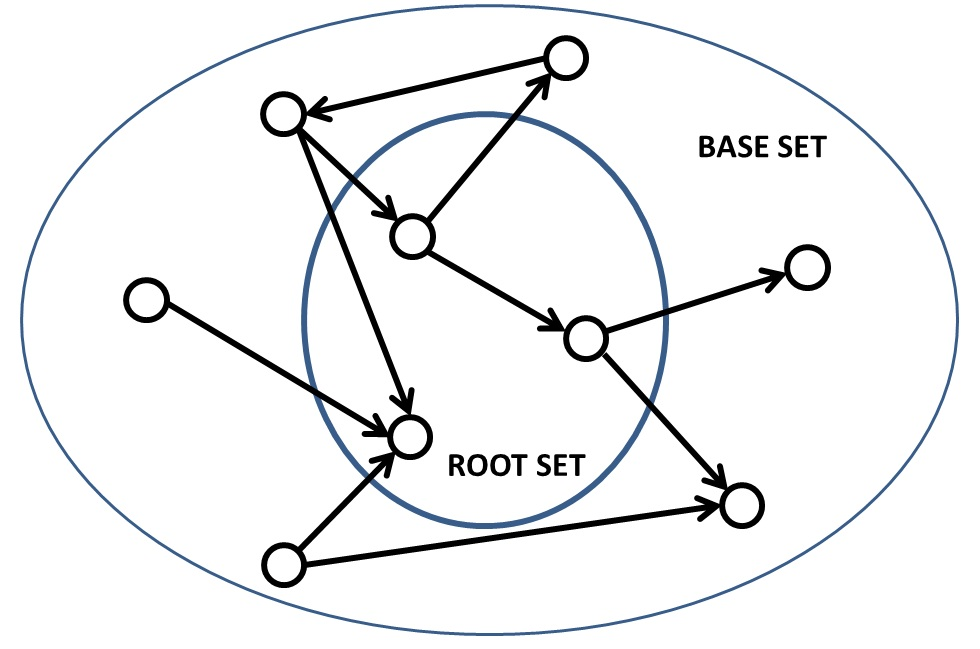
\includegraphics[width=5cm]{expanding_root.jpg}
\caption{Expanding the root set into the base set, taken from \cite{pict}}
\label{fig:HITS expanding}
\end{figure}
This expansion usually resolves the issue of synonyms, along with the issue that good authoritative pages may not contain the query item. The base set can become very large and so in practice a maximum number of inlinking and outlinking pages that are added for a particular node in the root set is fixed, for example at 100. 

The base set is constructed in this manner for several reasons, firstly a good authority page may not contain the query term  as there may be synonyms more commonly used. Also, if the root set contains a good hub set, this expansion means that the base set will then containing good authority pages that it may not have captured previously. The base set then forms the neighbourhood graph, N, which is then used in the computation of the authority and hub scores for all pages in N.


The first step in the weight-propagation step is the formation of the adjacency matrix \textbf{L}, where \[\textbf{L}_{ij} = \begin{cases} 1, & \textnormal{if there exists an edge from node \textit{i} to node \textit{j}}\\ 0 & \textnormal{otherwise}
\end{cases}\]
If we use the example in Figure \ref{fig:Example} as N for the following calculations, we are able to generate the following adjacency matrix:
\begin{equation*}
\textbf{L}=\left(
\begin{array}{cccccccc}
0 & 1 & 0 & 1 & 0 & 1 & 0 & 0 \\
0 & 0 & 1 & 0 & 1 & 0 & 0 & 0 \\
0 & 0 & 0 & 0 & 1 & 0 & 0 & 0 \\
0 & 0 & 0 & 0 & 1 & 0 & 1 & 0 \\
0 & 0 & 0 & 0 & 0 & 0 & 0 & 1 \\
0 & 0 & 0 & 1 & 0 & 0 & 1 & 1 \\
0 & 0 & 0 & 0 & 0 & 0 & 0 & 0 \\
0 & 0 & 0 & 0 & 1 & 0 & 1 & 0 \\
\end{array}
\right)
\end{equation*} 

We are able to represent Equations \eqref{eq:HITS1} in terms of this adjacency matrix as \begin{equation} \label{eq:HITSMatrix}
\textbf{x}^{(k)} = \textbf{L}^T\textbf{y}^{(k-1)}\quad\mathrm{and}\quad \textbf{y}^{(k)}=\textbf{Lx}^{(k)}
\end{equation} where \(\textbf{x}^{(k)}\) and \(\textbf{y}^{(k)}\) are $[\textit{n}\times 1]$ vectors which hold the approximate authority and hub scores at each iteration respectively. In the HITS algorithm, we first initialise $\textbf{y}^{(0)}$ = \textbf{e}, where \textbf{e} is the column vector of all ones, and then apply Equations \eqref{eq:HITSMatrix} until convergence. 

We are able to further simplify Equations \eqref{eq:HITSMatrix} to \begin{equation} \label{eq:HITSSimplify}
\textbf{x}^{(k)} = \textbf{L}^T\textbf{Lx}^{(k-1)}\quad\mathrm{and}\quad \textbf{y}^{(k)}=\textbf{LL}^T\textbf{y}^{(k-1)}
\end{equation} and this shows that we able to use the iterative power method on the matrices $\textbf{L}^T\textbf{L}$ and $\textbf{LL}^T$ respectively. The HITS algorithm defines the matrix $\textbf{L}^T\textbf{L}$ as the Authority matrix, and $\textbf{LL}^T$ as the Hub matrix. So when we apply the power method to these matrices, we compute the authority vector \textbf{x}, which contains the authority scores for all pages in the base set, and the hub vector, \textbf{y}, which similarly contains the hub scores.

Continuing to use Figure \ref{fig:Example} as our example, we are able to produce the following matrices;
\begin{equation*}
%\textnormal{Authority matrix} =
\textbf{L}^T\textbf{L}=\left(
\begin{array}{cccccccc}
0 & 0 & 0 & 0 & 0 & 0 & 0 & 0 \\
0 & 1 & 0 & 1 & 0 & 1 & 0 & 0 \\
0 & 0 & 1 & 0 & 1 & 0 & 0 & 0 \\
0 & 1 & 0 & 2 & 0 & 1 & 1 & 1 \\
0 & 0 & 1 & 0 & 4 & 0 & 2 & 0 \\
0 & 1 & 0 & 1 & 0 & 1 & 0 & 0 \\
0 & 0 & 0 & 1 & 2 & 0 & 3 & 1 \\
0 & 0 & 0 & 1 & 0 & 0 & 1 & 2 \\
\end{array}
\right)
\mathrm{,}\quad\mathrm{and}\quad
%\textnormal{Hub matrix} =
\textbf{LL}^T=\left(
\begin{array}{cccccccc}
3 & 0 & 0 & 0 & 0 & 1 & 0 & 0 \\
0 & 2 & 1 & 1 & 0 & 0 & 0 & 1 \\
0 & 1 & 1 & 1 & 0 & 0 & 0 & 1 \\
0 & 1 & 1 & 2 & 0 & 1 & 0 & 2 \\
0 & 0 & 0 & 0 & 1 & 1 & 0 & 0 \\
1 & 0 & 0 & 1 & 1 & 3 & 0 & 1 \\
0 & 0 & 0 & 0 & 0 & 0 & 0 & 0 \\
0 & 1 & 1 & 2 & 0 & 1 & 0 & 2 \\
\end{array}
\right)
\end{equation*} Where we note that these matrices are symmetric, positive semi-definite and non-negative, and so HITS with normalization will always converge, with as few as 5 iterations required in order to compute fairly accurate ranking lists \cite{manning}. 

Using the power method, as the Matlab code given in Appendix \ref{app:code}, we are able to compute authority score \textbf{x}, and hub score, \textbf{y}, vectors
\begin{eqnarray}
\textbf{x}^T = \left( \begin{array} {cccccccc}
0 & 0.030 & 0.069 & 0.118 & 0.343 &0.030 &0.305 &0.106
\end{array}\right) \\
\textbf{y}^T = \left( \begin{array} {cccccccc}
0.062 & 0.144 & 0.120 & 0.226 & 0.037 & 0.185 & 0 & 0.226
\end{array}\right)
\end{eqnarray} Hence we are able to produce two ranked lists for the user in terms of the authority and hub values of the pages in N, as shown in Table \ref{Table:HITS}.

\begin{table}[h] \caption{HITS Authority and Hub rankings}
 \centering
 \begin{tabular} {c| c c} 
 Node & Authority & Hub \\ [0.5ex] 
 \hline
 1&8&6\\
 2&6&4\\
 3&5&5\\
 4&3&1\\
 5&1&7\\
 6&6&3\\
 7&2&8\\
 8&4&1\\
 \end{tabular}
 \label{Table:HITS}
\end{table} 

We are able to note that node 5 is the most authoritative page, this follows from the fact that node 5 has many inlinks. Node 5 is also given a low hub score, as it points only into node 8, which has average authority in the graph. Subsequently, node 8 has a high hub score, as it points into the authoritative node 5.
 
\section{SALSA method} \label{sec:SALSA}
In 2000, Ronny Lempel and Schlomo Moran developed an algorithm for ranking web pages called the Stochastic Approach to Link Systems Analysis, SALSA, which incorporates ideas from both HITS and PR. Lempel and Moran developed SALSA as an attempt to avoid certain problems with HITS, such as topic drift \cite{bonato}. The algorithm is similar to HITS as it produces both authority and hub scores for the web pages in the graph, but SALSA examines random walks on two Markov chains derived from the web, similar to PR as opposed to a graph which is formed from connectivity analysis as in HITS \cite{lempel2000stochastic}, and the constructed graphs in SALSA gives higher authority weights than in HITS \cite{bonato}. SALSA is a query-dependant algorithm like HITS, however is less vulnerable to the TKC effect which can negatively impact rankings in HITS.

\subsection{SALSA Implementation}\label{sec:SALSA implementation}
The SALSA algorithm first forms a neighbourhood graph N in a similar method to HITS, see Section \ref{sec:HITS implementation} for more details, next a bipartite undirected graph, G, is formed. G is defined by three sets, $V_h$, the set of hub nodes, $V_a$, the set of authority nodes, and \textit{E}, which is the set of directed edges in N. Using Figure \ref{fig:Example} as an example, we find 
\[V_h = \{2,3,4,5,6,7,8\} \]
\[V_a = \{1,2,3,4,5,7,8\} \]
The bipartite graph for Figure \ref{fig:Example} is given in Figure \ref{fig:bipartite}, where the authority nodes are on the 'authority side' and similarly the hub nodes are on the 'hub side' of the graph. 

\begin{figure}[h!]
\centering
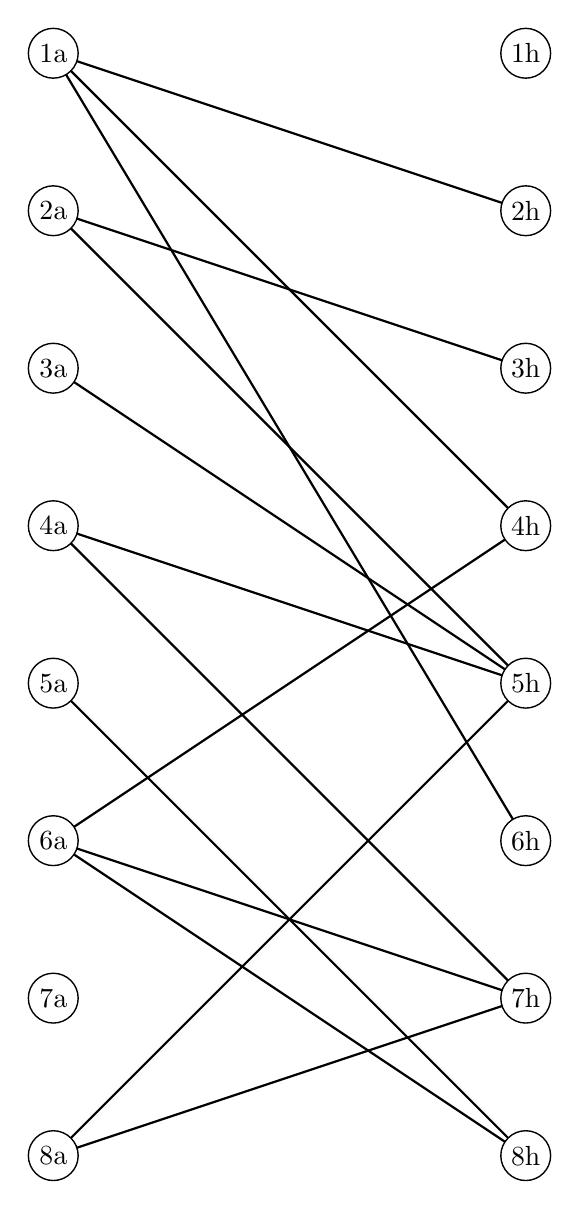
\begin{tikzpicture}
   \begin{scope}[rotate=90]
       \SetVertexNoLabel
       \grEmptyLadder[RA=2,RB=6]{8}   
       \AssignVertexLabel{a}{8h,7h,6h,5h,4h,3h,2h,1h}
       \AssignVertexLabel{b}{8a,7a,6a,5a,4a,3a,2a,1a}

   \end{scope} 
   \EdgeFromOneToSel{b}{a}{0}{1,3}
   \EdgeFromOneToSel{b}{a}{2}{0,1,4}
   \EdgeFromOneToSel{b}{a}{3}{0}
   \EdgeFromOneToSel{b}{a}{4}{1,3} 
   \EdgeFromOneToSel{b}{a}{5}{3}
   \EdgeFromOneToSel{b}{a}{6}{5,3}
   \EdgeFromOneToSel{b}{a}{7}{2,4,6} 
\end{tikzpicture}\caption{Bipartite graph of Figure \ref{fig:Example} } \label{fig:bipartite}
\end{figure}

The next step in the algorithm relates to the formation of the two Markov chains used, the authority Markov chain which has a transition probability matrix \textbf{A}, and a hub Markov chain with the matrix \textbf{H}. In relation to the SALSA algorithm \textbf{H} is the hub matrix, which is not to be confused with the hyperlink matrix that \textbf{H} represents in PR, as shown in Section \ref{sec:hyperlink}.  

{SALSA uses row and column weighting to calculate their authority and hub scores. Let $\textbf{L}_r$ be the adjacency matrix \textbf{L} with each non-zero row divided by the sum of the rows, and similarly $\textbf{L}_c$ is \textbf{L} where each non zero column is divided by the column sum.

\begin{equation*}
\textbf{L}=\left(
\begin{array}{cccccccc}
0 & 1 & 0 & 1 & 0 & 1 & 0 & 0 \\
0 & 0 & 1 & 0 & 1 & 0 & 0 & 0 \\
0 & 0 & 0 & 0 & 1 & 0 & 0 & 0 \\
0 & 0 & 0 & 0 & 1 & 0 & 1 & 0 \\
0 & 0 & 0 & 0 & 0 & 0 & 0 & 1 \\
0 & 0 & 0 & 1 & 0 & 0 & 1 & 1 \\
0 & 0 & 0 & 0 & 0 & 0 & 0 & 0 \\
0 & 0 & 0 & 0 & 1 & 0 & 1 & 0 \\
\end{array}
\right)
\end{equation*}

\begin{equation*} \renewcommand*{\arraystretch}{1.25}
\textbf{L}_r=\left(
\begin{array}{cccccccc}
0 & \frac{1}{3} & 0 & \frac{1}{3} & 0 & \frac{1}{3} & 0 & 0 \\
0 & 0 & \frac{1}{2} & 0 & \frac{1}{3} & 0 & 0 & 0 \\
0 & 0 & 0 & 0 & 1 & 0 & 0 & 0\\
0 & 0 & 0 & 0 & \frac{1}{2} & 0 & \frac{1}{2} & 0 \\
0 & 0 & 0 & 0 & 0 & 0 & 0 & 1 \\
0 & 0 & 0 & \frac{1}{3} & 0 & 0 & \frac{1}{3} & \frac{1}{3} \\
0 & 0 & 0 & 0 & 0 & 0 & 0 & 0 \\
0 & 0 & 0 & 0 & \frac{1}{2} & 0 & \frac{1}{2} & 0 \\
\end{array}
\right)
\mathrm{,}\qquad
\textbf{L}_c=\left(
\begin{array}{cccccccc} 
0 & 1 & 0 & \frac{1}{2} & 0 & 1 & 0 & 0 \\
0 & 0 & 1 & 0 & \frac{1}{4} & 0 & 0 & 0 \\
0 & 0 & 0 & 0 & \frac{1}{4} & 0 & 0 & 0 \\
0 & 0 & 0 & 0 & \frac{1}{4} & 0 & \frac{1}{3} & 0 \\
0 & 0 & 0 & 0 & 0 & 0 & 0 & \frac{1}{2} \\
0 & 0 & 0 & \frac{1}{2} & 0 & 0 & \frac{1}{3} & \frac{1}{2} \\
0 & 0 & 0 & 0 & 0 & 0 & 0 & 0 \\
0 & 0 & 0 & 0 & \frac{1}{4} & 0 & \frac{1}{3} & 0 \\
\end{array}
\right)
\end{equation*}

\textbf{H} is formed by removing the zero row and columns in $\textbf{L}_r\textbf{L}_c^T$, and similarly \textbf{A} is formed through removing the zero columns and rows in $\textbf{L}_c^T\textbf{L}_r$.

\begin{equation*} \renewcommand*{\arraystretch}{1.25}
\textbf{L}_r\textbf{L}_c^T=\left(
\begin{array}{cccccccc}
\frac{5}{6} & 0 & 0 & 0 & 0 & \frac{1}{6} & \textcolor{red}{0} & 0 \\
0 & \frac{5}{8} & \frac{1}{8} & \frac{1}{8} & 0 & 0 & \textcolor{red}{0} & \frac{1}{8} \\
0 & \frac{1}{4} & \frac{1}{4} & \frac{1}{4} & 0 & 0 & \textcolor{red}{0} & \frac{1}{4} \\
0 & \frac{1}{8} & \frac{1}{8} & \frac{7}{24} & 0 & \frac{1}{6} & \textcolor{red}{0} & \frac{7}{24} \\
0 & 0 & 0 & 0 & \frac{1}{2} & \frac{1}{2} & \textcolor{red}{0} & 0\\
\frac{1}{6} & 0 & 0 & \frac{1}{9} & \frac{1}{6} & \frac{4}{9} & \textcolor{red}{0} & \frac{1}{9} \\
\textcolor{red}{0} & \textcolor{red}{0} & \textcolor{red}{0} & \textcolor{red}{0} & \textcolor{red}{0} & \textcolor{red}{0} & \textcolor{red}{0} & \textcolor{red}{0} \\
0 & \frac{1}{8} & \frac{1}{8} & \frac{7}{24} & 0 & \frac{1}{6} & \textcolor{red}{0} & \frac{7}{24} \\
\end{array}
\right)
\mathrm{,}\qquad
\textbf{L}_c^T\textbf{L}_r=\left(
\begin{array}{cccccccc}
\textcolor{red}{0} & \textcolor{red}{0} & \textcolor{red}{0} & \textcolor{red}{0} & \textcolor{red}{0} & \textcolor{red}{0} & \textcolor{red}{0} & \textcolor{red}{0} \\
\textcolor{red}{0} & \frac{1}{3} & 0 & \frac{1}{3} & 0 & \frac{1}{3} & 0 & 0 \\
\textcolor{red}{0} & 0 & \frac{1}{2} & 0 & \frac{1}{2} & 0 & 0 & 0 \\
\textcolor{red}{0} & \frac{1}{6} & 0 & \frac{1}{3} & 0 & \frac{1}{6} & \frac{1}{6} & \frac{1}{6} \\
\textcolor{red}{0} & 0 & \frac{1}{8} & 0 & \frac{5}{8} & 0 & \frac{1}{4} & 0 \\
\textcolor{red}{0} & \frac{1}{3} & 0 & \frac{1}{3} & 0 & \frac{1}{3} & 0 & 0 \\
\textcolor{red}{0} & 0 & 0 & \frac{1}{9} & \frac{1}{3} & 0 & \frac{4}{9} & \frac{1}{9} \\
\textcolor{red}{0} & 0 & 0 & \frac{1}{6} & 0 & 0 & \frac{1}{6} & \frac{2}{3} \\
\end{array}
\right)
\end{equation*}
 Hence we are able to form the SALSA hub and authority matrices for the example;
\begin{equation*} \renewcommand*{\arraystretch}{1.25}
\textbf{H}=\left(
\begin{array}{ccccccc}
\frac{5}{6} & 0 & 0 & 0 & 0 & \frac{1}{6} & 0 \\
0 & \frac{5}{8} & \frac{1}{8} & \frac{1}{8} & 0 & 0 & \frac{1}{8} \\
0 & \frac{1}{4} & \frac{1}{4} & \frac{1}{4} & 0 & 0 & \frac{1}{4} \\
0 & \frac{1}{8} & \frac{1}{8} & \frac{7}{24} & 0 & \frac{1}{6} & \frac{7}{24} \\
0 & 0 & 0 & 0 & \frac{1}{2} & \frac{1}{2} & 0\\
\frac{1}{6} & 0 & 0 & \frac{1}{9} & \frac{1}{6} & \frac{4}{9} & \frac{1}{9} \\
0 & \frac{1}{8} & \frac{1}{8} & \frac{7}{24} & 0 & \frac{1}{6} & \frac{7}{24} \\
\end{array}
\right)
\mathrm{,}\quad\mathrm{and}\quad
\textbf{A}=\left(
\begin{array}{ccccccc}
\frac{1}{3} & 0 & \frac{1}{3} & 0 & \frac{1}{3} & 0 & 0 \\
0 & \frac{1}{2} & 0 & \frac{1}{2} & 0 & 0 & 0 \\
\frac{1}{6} & 0 & \frac{1}{3} & 0 & \frac{1}{6} & \frac{1}{6} & \frac{1}{6} \\
0 & \frac{1}{8} & 0 & \frac{5}{8} & 0 & \frac{1}{4} & 0 \\
\frac{1}{3} & 0 & \frac{1}{3} & 0 & \frac{1}{3} & 0 & 0 \\
0 & 0 & \frac{1}{9} & \frac{1}{3} & 0 & \frac{4}{9} & \frac{1}{9} \\
0 & 0 & \frac{1}{6} & 0 & 0 & \frac{1}{6} & \frac{2}{3} \\
\end{array}
\right)
\end{equation*}

Both the authority and the hub matrix are primitive, as the Markov chains for both are aperiodic \cite{lempel2000stochastic}. If G is connected, then \textbf{H} and \textbf{A} are both irreducible Markov chains, and we are able to find the stationary vector, $\boldsymbol\pi_h^T$, of \textbf{H} which gives the hub scores for N. Equivalently $\boldsymbol\pi_a^T$, the stationary vector of \textbf{A} gives the authority scores. By the ergodic theorem \cite{gallager1992discrete}, we can find the  the stationary distribution of the underlying Markov chain, as this is the principal eigenvector of an irreducible, aperiodic, stochastic matrix. The entries with the highest entries relate the the nodes that are most frequently visited by the (infinite) random walk. 

In our example, G in Figure \ref{fig:bipartite} is not connected, as we are not able to reach nodes 7a and 1h though any of the other nodes. Due to this, our \textbf{H} and \textbf{A} matrices contain multiple connected graphs. \textbf{H} contains two connected sets, \textit{X} = \{7\}, and \textit{Y}=\{1,2,3,4,5,6,8\}, \textbf{A} also contains two sets, \textit{W}=\{1\} and \textit{Z}=\{2,3,4,5,6,7,8\}, we are able to compute the stationary values for these connected sets through the use of the power method, as discussed in Section \ref{sec:solve}.

The stationary vectors, $\boldsymbol\pi_h^T$, for the two Markov chains which make up the Hub Markov chain is \textit{X} and \textit{Y} are 
\[\boldsymbol\pi_h^T (X) = \begin{blockarray}{c}
7 \\
\begin{block}{(c)}
 1 \\
\end{block}
\end{blockarray} \mathrm{,}\quad\mathrm{and}\quad
\boldsymbol\pi_h^T (Y) =
\begin{blockarray}{ccccccc}
1 & 2 & 3 & 4 & 5 & 6 & 8 \\
\begin{block}{(ccccccc)}
 0.214 & 0.143 & 0.071 & 0.143 & 0.071 & 0.214 & 0.143 \\
\end{block}
\end{blockarray} \] correspondingly the stationary values for the two components in \textbf{A} are
\[\boldsymbol\pi_a^T (W) = \begin{blockarray}{c}
1 \\
\begin{block}{(c)}
 1 \\
\end{block}
\end{blockarray} \mathrm{,}\quad\mathrm{and}\quad
\boldsymbol\pi_a^T (Z) = \begin{blockarray}{ccccccc}
2 & 3 & 4 & 5 & 6 & 7 & 8 \\
\begin{block}{(ccccccc)}
0.071 & 0.071 & 0.143 & 0.286 & 0.071 & 0.214 & 0.143 \\
\end{block}
\end{blockarray}\]
From these components we are able to calculate the local Hub and Authority rankings:
\[\boldsymbol\pi_h^T (X) = \begin{blockarray}{c}
7 \\
\begin{block}{(c)}
 1 \\
\end{block}
\end{blockarray} \mathrm{,}\quad\mathrm{and}\quad
\boldsymbol\pi_h^T (Y) =
\begin{blockarray}{ccccccc}
1 & 2 & 3 & 4 & 5 & 6 & 8 \\
\begin{block}{(ccccccc)}
1 & 3 & 6 & 3 & 6 & 1 & 3 \\
\end{block}
\end{blockarray} \]
\[\boldsymbol\pi_h^T (W) = \begin{blockarray}{c}
1 \\
\begin{block}{(c)}
 1 \\
\end{block}
\end{blockarray} \mathrm{,}\quad\mathrm{and}\quad
\boldsymbol\pi_h^T (Z) = \begin{blockarray}{ccccccc}
2 & 3 & 4 & 5 & 6 & 7 & 8 \\
\begin{block}{(ccccccc)}
5 & 5 & 3 & 1 & 5 & 2 & 3  \\
\end{block}
\end{blockarray} \]

We are now able to calculate the global Hub and Authority scores, this is done by weighting the local scores by the proportion of G that they contain, for example \textit{X} contains $\frac{1}{8}$ of the nodes in the hub set, and so SALSA proposes that the $\boldsymbol\pi_h^T(X)$ vector should be weighted by $\frac{1}{8}$. This leads to the global scores;
\begin{eqnarray*}
\pi_h = \left( \begin{array} {cccccccc}
0.188 & 0.125 & 0.063 & 0.125 & 0.063 & 0.188 & 0.125 & 0.125
\end{array}\right) \\
\pi_a = \left( \begin{array} {cccccccc}
0.125 & 0.063 & 0.063 & 0.125 & 0.250 & 0.063 & 0.188 & 0.125
\end{array}\right)
\end{eqnarray*} as shown in Table \ref{Table:SALSA}

\begin{table}[H] \caption{SALSA Authority and Hub rankings}
 \centering
 \begin{tabular} {c| c c} 
 Node & Authority & Hub \\ [0.5ex] 
 \hline
 1&3&1\\
 2&6&3\\
 3&6&7\\
 4&3&3\\
 5&1&7\\
 6&6&1\\
 7&2&3\\
 8&2&3\\
 \end{tabular}
 \label{Table:SALSA}
\end{table}

\section{Comparing PageRank, HITS and SALSA} \label{sec:compare}
\subsection{Spamdexing}
Spamdexing is an intentional attempt to improve the ranking of a page on a SE, this can be done by link spam or by link farms, as shown in Figure \ref{fig:link farm}. 
\begin{figure}[h!]
\centering
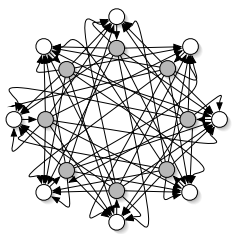
\includegraphics[width=5cm]{link_farm_baldi.png}
\caption{A link farm, where the shaded nodes are all copied of the same page, taken from \cite{baldi2003modeling}}
\label{fig:link farm}
\end{figure}

PR is sensitive to in-degree and so a simple way to spamdex PR is to increase the in-degree to your page. \cite{bonato} As HITS and SALSA are less sensitive to spamdexing than PR. 

\subsection{Dual Rankings}
An advantage of HITS compared to PR is the dual ranking that is assigned to each web page, a user might find this useful to find out which pages are the most authoritative on a query topic.

SALSA also has dual rankings as does HITS, and is also query dependant, making it computationally less taxing than PR \cite{langville}.


\subsection{Query-dependence}
HITS is also query-dependant, it first generates a root set dependant on the query, and returns two real numbers for a given page HITS deems relevant to the topic, however PR returns a rank for each page in the whole web graph, this is also a weakness of the algorithm, as the computation required to produce the dual rankings must occur at query time. It is possible to make HITS query dependant by removing the sampling step of the algorithm, hence reducing computation time. 

\subsection{Uniqueness}
A problem can arise with the uniqueness of the vectors produced, as different authority and hub vectors are computed by different choices of the initial vector \cite{langville}. Output of HITS depends on weather the implementation uses the initial authority or hub vector \cite{farahat2006authority}. HITS converges to a non-unique solution as the authority matrix is not irreducible, we are able to modify HITS in a manner similar to the primitivity adjustment in PR, as discussed in section \ref{sec:matrix}. In this modification, we can create a modified authority matrix \(\xi\textbf{L}^T\textbf{L} +\frac{(1-\xi)}{n}\textbf{ee}^T\) can be created, where $0<\xi<1$ \cite{ng2001stable}, and similarly create a hub matrix, \(\xi\textbf{LL}^T +\frac{(1-\xi)}{n}\textbf{ee}^T\) . These modified matrices are now irreducible, and by the Perron-Frobenius theorem, we can find a unique, normalised, positive dominant eigenvector \cite{meyer2000matrix}. This adjustment also solves the problem arising with pages having the same rank, for example in Table \ref{Table:HITS}, nodes 2 and 6 both have the same rank in terms of their authority.

SALSA can give inconsistent hub and authority rankings due to non-uniqueness \cite{farahat2006authority}.

HITS and SALSA eigenvectors do not have to be unique, whereas for PR they do. HITS and SALSA can now behave unexpectedly, as the output depends on the initial seed vector, PR doesn't display this inconsistency \cite{farahat2006authority}. A ranking algorithm that assigns both hub and authority weights is badly behaved on G if the final results is dependant on on initial vectors, or if a node is given authority or hub weight of zero, even if it has either an in-degree or out-degree which is greater than zero \cite{bonato}. %This occurs in our example at nodes 2h and 6h, they are given an in-link weight of zero, as the only in-link is from node 1a, which also has a weight of 0.  

\subsection{Topic Drift}

Topic drift has been shown to be avoided by using topic vectors to filter N, a topic vector is a term vector which has been computed from the text of pages in the base set, a page is only able to remain in N if its term vector is a good match to this topic vector. \textcolor{red}{\textbf{EXPLAIN MORE HERE}}

SALSA, is less impacted by topic drift \cite{lempel2000stochastic}, and is less susceptible to spamming, the coupling between the hub and authority scores is less strict in SALSA. However HITS and SALSA are easier to spam than PR due to the mutual reinforcement effect \cite{langville}. 

\subsection{Computation costs}
A weakness of PR is that the web contains many documents that calculations must be done on many computers, also the structure and content of the web changes daily, leading to the 'Google Dance' which must be done monthly \cite{thorson2004modeling}. 

HITS is usually described as running on a smaller collection of articles that have been retrieved on a query topic, whilst PR runs on the entire web \cite{ng2001link}. As we form \textbf{L} through the base set, the order of \textbf{L} is much smaller then the total number of pages on the web, and so the computation required in producing a ranked list of the web pages is less costly than the computation in PR, we also do not need to compute eigenvectors for both matrices, as we are able to use the equations, which is also computationally simpler. 

Figure \ref{fig:N build} shows how the N graph that is built through the HITS algorithm is smaller than the web graph, and so it is less computationally taxing on a system.

\begin{figure}[h] 
\centering
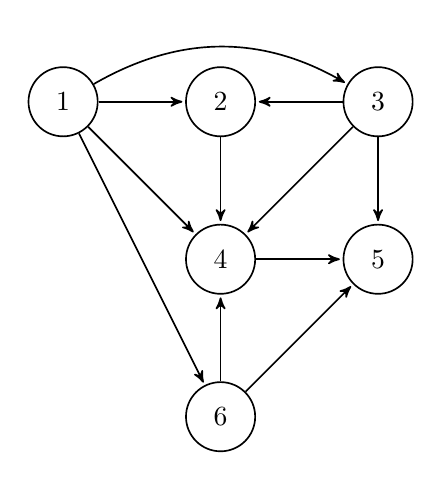
\begin{tikzpicture}[->,>=stealth',shorten >=1pt,auto,node distance=2cm,
semithick]
\tikzstyle{every state}=[fill=white,draw=black,text=black]
\node[state] (1) {$1$};
\node[state] (2) [right of=1] {$2$};
\node[state] (3) [right of=2] {$3$};
\node[state] (4) [below of=2] {$4$};
\node[state] (5) [below of=3] {$5$};
\node[state] (6) [below of=4] {$6$};
\path (1) edge node{} (2)
          edge [bend left] node{} (3)
          edge node{} (4)
          edge node{} (6)
      (2) edge node{} (4)
      (3) edge node{} (2)
          edge node{} (4)
          edge node{} (5)
      (4) edge node{} (5)
      (6) edge node{} (5)
          edge node{} (4);
\end{tikzpicture} \qquad\qquad
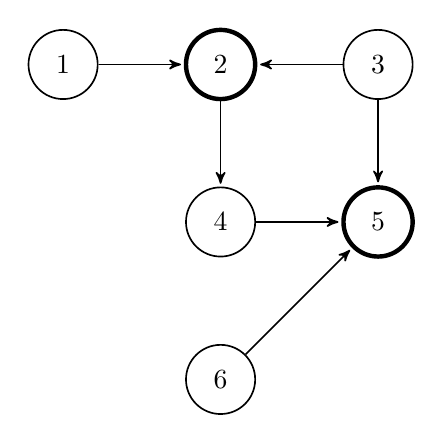
\begin{tikzpicture}[->,>=stealth',shorten >=1pt,auto,node distance=2cm,
semithick]
\tikzstyle{every state}=[fill=white,draw=black,text=black]
\node[state] (1) {$1$};
\node[state] (2) [ultra thick, right of=1] {$2$};
\node[state] (3) [right of=2] {$3$};
\node[state] (4) [below of=2] {$4$};
\node[state] (5) [ultra thick, below of=3] {$5$};
\node[state] (6) [below of=4] {$6$};
\path (1) edge node{} (2)
      (2) edge node{} (4)
      (3) edge node{} (2)
          edge node{} (5)
      (4) edge node{} (5)
      (6) edge node{} (5);
\end{tikzpicture}
\caption{Neighbourhood graph, N,  for {2,5}} \label{fig:N build}
\end{figure}


\subsection{TKC Effect}
There are three main problems which can arise through using connectivity analysis on web pages, such as mutually reinforced relationships in a tightly knitted community, TKC, where a set of documents on page A could point to a single document on page B which would then drive up the hub score of page A, whilst increasing the authority ranking on page B, when this occurs in the TKC, pages that may have no authority on a topic or may pertain to just one aspect of the query may score high undeservedly \cite{lempel2000stochastic}. There is also a problem of automatically generated links, which would not represent human opinion, also topic-drift arises through the usage of connectivity analysis, where when building N, it is possible for an authoritative page which is off-topic can be linked to pages which contain the query term, and so can skew the rankings to off-topic pages. The general solution to this problem as suggested by Bharat and Herzinger is to use content analysis \cite{bharat1998improved}. Using this improved algorithm, precision over the original HITS algorithm has been shown to increase by 45\%, however this is limited to topics that are already well-represented and connected on the web. 

'It is this combination of a site’s intra-community authority score and its community’s size that allows the stochastic approach to blend authorities from different aspects of a multi-topic query, and which reduces its vulnerability to the TKC effect.We have shown that the ranking produced by SALSA is equivalent to a weighted in=out-degree ranking (with the sizes of irreducible components also playing a part). This makes SALSA computationally lighter than the mutual reinforcement approach. We note that SALSA is less vulnerable to the TKC effect, and produces good results in many cases where the mutual reinforcement approach fails to do so.\cite{lempel2000stochastic}'

HITS emphasises the mutual reinforcement between authority and hub web pages, whereas PR focuses more on web surfing based on random walk models HITS emphasises the mutual reinforcement between authority and hub web pages \cite{ding2003pagerank}.

\subsection{Sensitivity}

HITS is insensitive to minor changes in its neighbourhood graph, N, PR can be sensitive depending on where the change occurred. If the change in the web graph occurred with pages that have a low PR value, then the overall PR is very small \cite{bonato}.


\begin{table}[H] \caption{Page rankings for Figure \ref{fig:Example} using PR, HITS and SALSA }
 \centering
 \begin{tabular} {c| c| c| c| c| c} 
 \multirow{2}{*}{Node} & \multirow{2}{*}{PR} & \multicolumn{2}{|c|}{HITS} & \multicolumn{2}{|c}{SALSA} \\ [0.5ex] 
 {}&{}&Authority & Hub & Authority & Hub\\ 
 \hline
 1&8&8&6&3&1\\
 2&6&6&4&6&3\\
 3&5&5&5&6&7\\
 4&4&3&1&3&3\\
 5&2&1&7&1&7\\
 6&6&6&3&6&1\\
 7&3&2&8&2&3\\
 8&1&4&1&2&3\\
 \end{tabular}
 \label{Table: comparison}
\end{table}

%--------------------Improvements
\chapter{Improvements to the PageRank Algorithm} \label{chap:Improve}

In this chapter we will discuss various methods of improving the PageRank algorithm in order to improve the accuracy of the PageRank vector for a user. The original algorithm is simplistic in the assumption that a random surfer will move throughout the hyperlink graph without any bias, and so it is not very realistic, as a surfer will be more drawn to pages that interest them specifically, we will discuss this more with respect to the formulation of a Topic-specific PageRank algorithm. Another modified algorithm is the Weighted PageRank which takes into account the importance of the outlinks and inlinks a page has \cite{xing2004weighted}. We can also use Weighted Links Rank, WL Rank, which considers different web page attributes to give different weights to some links, this algorithm gives more weight to links at the beginning of pages \cite{baeza2004web}.

\section{Intelligent Surfer} \label{sec:intelligent}
PageRank as an algorithm ranks a page highly if it is at the centre of a hyper graph, however the highest ranked pages should also be relevant to the query. We can solve this by the PageRank algorithm by the use of an intelligent surfer as opposed to a random surfer. The intelligent surfer will be more likely to jump to a more content-filled page, and so these pages should be assigned a greater weight \cite{langville}. In practice, the hyperlink matrix could be formed from using access logs in order to find the tendencies of the surfer. 

The use of an intelligent surfer outperforms the standard PageRank algorithm in terms of the quality of the pages, whilst still being efficient enough in terms of being a practical search engine \cite{richardson2002intelligent}. 

This algorithm can be viewed as a solution to topic drift, as discussed in Section \ref{sec:HITS}, as only relevant topics will be  given. In order to ensure that the algorithm is efficient, the majority of the computation is performed at crawl time, rather than at query time \cite{richardson2002intelligent}. 

\section{Weighted PageRank}\label{sec:weighted}
Weighted PageRank algorithm differs from the standard algorithm by assigning more value to important pages rather than diving the rank equally, as each outlink page receives a value which is proportional to its popularity \cite{xing2004weighted}. $W^{in}_{(j,i)}$ is the weight of the link between pages \textit{i} and \textit{j}, which is calculated as 
\begin{equation}\label{eq:weightin}
W^{in}_{(j,i)} = \frac{I_i}{\sum_{k\in R(i)}I_k}
\end{equation}
where $I_i$ and $I_k$ represent the number of inlinks of pages \textit{i} and \textit{j} respectively, and $R(j)$ is the set of pages that \textit{j} links into. 
Similarly $W^{out}_{(j,i)}$ is calculated as
\begin{equation}\label{eq:weightout}
W^{out}_{(j,i)} = \frac{O_i}{\sum_{k\in R(i)}O_k}
\end{equation}

In the example Figure \ref{fig:Example}, Page 2 has 2 outlinks, 3 and 5. The inlinks and outlinks of these pages are, $I_3 = 1$, $I_5 = 4$, $O_3 = 1$ and $O_5 = 1$, and so we can calculate 
\[W^{in}_{(2,3)} = \frac{I_3}{I_3 + I_5} = \frac{1}{5} \]
and 
\[W^{out}_{(2,3)} = \frac{O_3}{O_3 + O_5} = \frac{1}{2} \] 

The original PageRank formula given in Equation \eqref{eq:power H}, is now modified to 
\begin{equation} \label{eq:WPR formula}
\boldsymbol\pi^{(k+1)T} = \boldsymbol\pi^{(k)T}\textbf{H}
\end{equation}
When Equation \eqref{eq:weightin} and Equation \eqref{eq:weightout} applied to Figure \ref{fig:Example}, we produce a hyperlink matrix which is different to \textbf{H} produced in section \ref{sec:hyperlink}. 

\[\textbf{W}_{out}=\left(
\begin{array}{cccccccc}
0 & \frac{2}{7} & 0 & \frac{2}{7} & 0 &\frac{3}{7} & 0 & 0 \\
0 & 0 &\frac{1}{2}& 0 &\frac{1}{2}& 0 & 0 & 0\\
0 & 0 & 0 & 0 & 1 & 0 & 0 & 0\\
0 & 0 & 0 & 0 & 1 & 0 & 0 & 0\\
0 & 0 & 0 & 0 & 0 & 0 & 0 & 1\\
0 & 0 & 0 & \frac{1}{2} & 0 & 0 & 0 & \frac{1}{2} \\
0 & 0 & 0 & 0 & 0 & 0 & 0 & 0\\
0 & 0 & 0 & 0 & 1 & 0 & 0 & 0\\
\end{array}
\right) \mathrm{,}\quad\mathrm{and}\quad\textbf{W}_{in}=\left(
\begin{array}{cccccccc}
0 & 0 & 0 & 0 & 0 & 0 & 0 & 0 \\
0 & 0 & 0 & 0 & 0 & 0 & 0 & 0\\
0 & 1 & 0 & 0 & 0 & 0 & 0 & 0\\
0 & 0 & 0 & 0 & 0 & 1 & 0 & 0\\
0 & \frac{1}{6} & \frac{1}{6} & \frac{1}{3} & 0 & 0 & 0 & \frac{1}{3}\\
0 & 0 & 0 & 0 & 0 & 0 & 0 & 0 \\
0 & 0 & 0 & \frac{2}{5} & 0 & \frac{1}{5} & 0 & \frac{2}{5}\\
0 & 0 & 0 & 0 & \frac{4}{5} & \frac{1}{5} & 0 & 0\\
\end{array}
\right)	\]
\[\textbf{H}_{WPR}=\left(
\begin{array}{cccccccc}
0 & 0 & 0 & 0 & 0 & 0 & 0 & 0 \\
0 & 0 & 0 & 0 & 0 & 0 & 0 & 0\\
0 & 0 & \frac{1}{2} & 0 & \frac{1}{2} & 0 & 0 & 0\\
0 & 0 & 0 & \frac{1}{2} & 0 & 0 & 0 & \frac{1}{2}\\
0 & 0 & \frac{1}{12} & 0 & \frac{11}{12} & 0 & 0 & 0\\
0 & 0 & 0 & 0 & 0 & 0 & 0 & 0 \\
0 & 0 & 0 & \frac{1}{10} & \frac{8}{10} & 0 & 0 & \frac{1}{10}\\
0 & 0 & 0 & \frac{1}{10} & 0 & 0 & 0 & \frac{9}{10}\\
\end{array}
\right)	\]

Through the same methods as discussed in chapters 2 and 3, we produce a PageRank vector 
\[\boldsymbol\pi_{WPR} = \left(
\begin{array}{c}
0.028 \\
0.028 \\
0.097 \\
0.097 \\
0.395 \\
0.028 \\
0.028 \\
0.302
\end{array}
\right)\]
when we compare the PageRankings produced by performing the standard algorithm and the weighted algorithm:
\begin{table}[H] \caption{Comparison of PageRankings produced by standard algorithm and the weighted PageRank algorithm}
 \centering
 \begin{tabular} {c| c c} 
 Node & PR & WPR \\ [0.5ex] 
 \hline
 1&8&5\\
 2&6&5\\
 3&5&3\\
 4&4&3\\
 5&2&1\\
 6&6&5\\
 7&3&5\\
 8&1&2\\
 \end{tabular}
 \label{Table:WPR and PR}
\end{table}
\cite{langville}, \cite{baeza2004web}

The WPR algorithm has been shown as being able to identify a greater number of relevant pages when compared to the standard PR algorithm \cite{xing2004weighted}. We will also use the WPR algorithm later in this report in section \ref{sec:Roads}, in order to predict the human movement in an urban space. 

\section{Personalization Vector} \label{sec:Personalization}
We are able to form a personalised PR which 'can create a view of Web from a particular perspective' \cite{page1999pagerank}. We can do this by using $\textbf{ev}^T$ in the general PR algorithm instead of $\frac{1}{n}\cdot1^T$, and so the Google matrix in Equation \eqref{eq:G} is now given as \begin{equation}\label{eq:Personalisation G}
\textbf{G}=\alpha\textbf{S}+\left((1-\alpha)\cdot\textbf{ev}^T\right)
\end{equation} and so we are able to state the PR equation Equation \eqref{eq:power to G} as; 
\begin{align}
\boldsymbol{\pi}^{(k+1)T} &= \boldsymbol{\pi}^{(k)T}\textbf{G} \nonumber \\
&= \alpha\boldsymbol{\pi}^{(k)T}\textbf{S} + (1-\alpha)\boldsymbol{\pi}^{(k)T}\textbf{ev}^T \nonumber \\
&= \alpha\boldsymbol{\pi}^{(k)T}\textbf{H} + \left(\alpha\boldsymbol{\pi}^{(k)T}\textbf{a} + 1 - \alpha\right)\textbf{v}^T \label{eq:Power personalization}
\end{align}
When we use this personalization vector, the probabilities are no longer uniformly distributed \cite{langville}. This personalization vector is an arbitrary stochastic vector \cite{bonato}. The use of the personalization vector retains the advantage of being able to use the power method in order to compute the rankings, along with maintaining the other advantages of PR such as the minimal storage required in order to generate the rankings.

Personalized PR changes only the PR vector itself, as different personalizations produce different rankings \cite{thorson2004modeling}. The personalization vector can be used to control spamming by link farms, as PR is vulnerable to this spamdexing as discussed in Section \ref{sec:compare}, \cite{thorson2004modeling}. However personalized PR is costly in implementation as it is very difficult to form the personalization vector, and so in order to combat this we use pseudo-personalization PR systems, such as Topic-Specific PageRank.

\subsection{Topic Specific PageRank} \label{sec:Topic specific PR}
Haveliwala suggested a pseudo-personalised PR algorithm known at Topic-Specific PageRank,TSPR, which aims to group users in order to lessen the computation of unique personalised PR for each user \cite{haveliwala2002topic}. This is done by biasing the PR vectors created to a set of representative topics \cite{haveliwala2002topic}, where the bias PR vectors are calculated prior to query time \cite{langville}, this biasing involves the introduction of artificial links into the web graph. The biases are applied during iterations to increase the importance of certain categories and pages \cite{haveliwala1999efficient}. The use of the TSPR generates more accurate ranking than the single generic PR vector, as a certain user will be more interested in some topics, and so intuitively these pages should have a higher ranking. 

TSPR is similar to HITS, as discussed in Section \ref{sec:HITS}, as it is a query-dependant algorithm, which allows the query to impact the ranking, however like PR there is minimal query-time processing. 

TSPR is also less vulnerable to topic drift, as we avoid the problem of heavily linked web pages having a high ranking for queries that they have little authority. 

TSPR suggests that the web page can be represented sufficiently by 16 main topics;
\begin{enumerate}
\item Arts
\item Business
\item Computers
\item Games
\item Health
\item Home
\item Kids \& teens
\item News
\item Recreation
\item Reference
\item Regional
\item Science
\item Shopping
\item Society
\item Sports
\item World
\end{enumerate} During the offline crawl, 16 TSPR vectors are created from information supplied by the user. This information can be created automatically from an analysis of the bookmarks and browser history over time, or the user could manually input their preference for each topic, the algorithm assumes that an individuals interest can be approximated sufficiently as a linear combination of the smaller topic page distributions \cite{manning}.
\begin{figure}[h!]
\centering
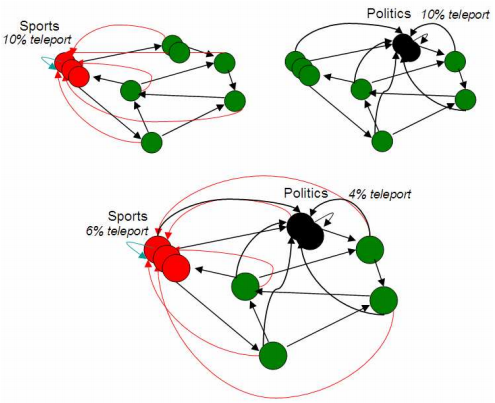
\includegraphics[width=10cm]{Topic-specific_PageRank_Manning.png}
\caption{Topic-specific PageRank, where a user has 60\% interest in sports, and 40\% interest in politics, taken from \cite{manning}}
\label{fig:topic-specific}
\end{figure}

In Figure \ref{fig:topic-specific}, $\alpha$ is 0.9, the user will teleport 6\% to sports pages, and 4\% to politics pages.

At query time, the algorithm calculated the similarity of the query (including the user context if available) to each of these topics, and then takes a linear combination of the TSPR vectors weighted with respect to the similarity of the query (and context) to the topic. As the computation of the TSPR is done prior to query-time, the algorithm doesn't have large query-time costs \cite{haveliwala2002topic}.  The TSPR vectors are denoted as $\boldsymbol{\pi}_t$ where \textit{t} denotes the topic, for example the sports PageRank vector would be $\boldsymbol{\pi}_s$, each user would have a mixture of interests, for example User P could be interested in sports 60\%, but also interested in politics 40\%, and so the TSPR would be $\boldsymbol{\pi}_P=0.6\pi_s+0.4\pi_p$, this would lead to a Markov chain with a steady state distribution that has been personalized. 


Forms a topic-sensitive, query-dependant PR vector which is a convex combination of PR vectors \cite{langville}. This uses a bayesian classifier in order to compute the $\beta_i$'s for the experiments \cite{langville}.   The implementation of TSPR is costly as for each user there is a need to compute a unique transition matrix \cite{manning}. 

%--------------------Applications
\chapter{Applications of the PageRank algorithm} \label{chap:Applications}

The PR algorithm can also be used in many varied applications beyond ranking web pages \cite{gleich2015pagerank}, which we explore in this chapter. We will explore the algorithm with respect to modelling traffic in Durham in more detail, alongside applications in chemistry and in recommender systems. 

The PR algorithm can be used as a measure of network centrality, where you are able to understand a graph better when PageRank reveals what is most important. We are also able to apply modified PR to some applications, for example reverse PR can be used to model food chains, where a species,\textit{i}, is important if it feeds a species, \textit{j} \cite{allesina2009googling}. 

\section{Wikipedia} \label{sec:wiki}
We are able to apply PR to large databases such as Wikipedia, for example, we can generate reading lists for university courses automatically from exploiting the link structure of Wikipedia \cite{wissner2006preparation}. We are able to rank articles to find the top 100 historical figures and which cultures have the largest reach, for example a culture will have a high PR if it has many inlinks from other cultures. PR reveals that Carl Linnaeus is the most 'important' page due to the fact that he developed the scientific classification system we use for animals, insects and plants, and so these pages link back to him \cite{eom2015interactions}. We are also able to conclude that the most important figures in history are Western men who are born after the 17th Century. This mathematical analysis of historical figures and cultures using Wikipedia can be very useful in exploring interactions between world cultures and understanding history.


\section{Chemistry} \label{sec:chem}
The PR algorithm has been used when studying molecules in chemistry, specifically in MoleculaRnetworks \cite{JCC:JCC22917}, which is a toolkit for identifying a shape of a solvent and exploring the H-bonding in that solvent. 
\begin{figure}
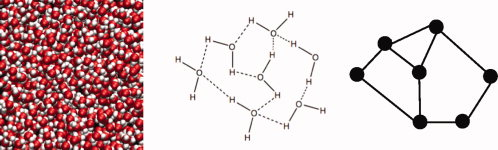
\includegraphics[width=\linewidth]{Decomposition_of_simulation_date_into_a_graph_-chem.jpg}
\caption{Decomposition of simulation data into a graph, taken from \cite{JCC:JCC22917}}
\label{fig:chem}
\end{figure}
We are able to assess changes to the Hydrogen bond network due to the solute through the analysis of the network structure, as a graph is formed where the nodes are water molecules, and links represent potential hydrogen bonds, as shown in Figure \ref{fig:chem}. PageRank of each water molecule is determined by the number of edges connected to it, along with the number of edges connected to the nodes neighbours. As each polyhedron has its own unique PR vector, we are able to access a database in order to confirm the polyhedra structure. The use of PageRank is a novel way to extract chemical information, and can enhance the traditional methods used in chemical spectroscopy.

\section{Recommender Systems} \label{sec:recommender}
PR can modified so that it can be used in recommender systems for companies such as Netflix or Amazon, this modified PR is ItemRank \cite{gleich2015pagerank}. ItemRank makes personalised product suggestions by extracting knowledge for the users prior interactions \cite{gori2007itemrank}. ItemRank is a random-walk based algorithm where users rate the items, and they wish to be recommended items that have been rated highly, and has been shown to perform better than over algorithms whilst being less complex \cite{gori2007itemrank}.

\section{Roads and Urban Networks} \label{sec:Roads}
We are able to apply the PageRank algorithm to road networks in order to predict traffic flow and also human movement. Jiang et al. found that Weighted PageRank, as discussed in Section \ref{sec:weighted} of this report, is the best metric with regards to correlating or predicting traffic flow \cite{1742-5468-2008-07-P07008}. A city can be topologically represented by a connectivity graph as shown in Figure \ref{fig:city rep}, and as over 60\% of human movement can be predicted or explained using a connectivity graph \cite{doi:10.1080/13658810802022822}.

\begin{figure}[h!]
\centering
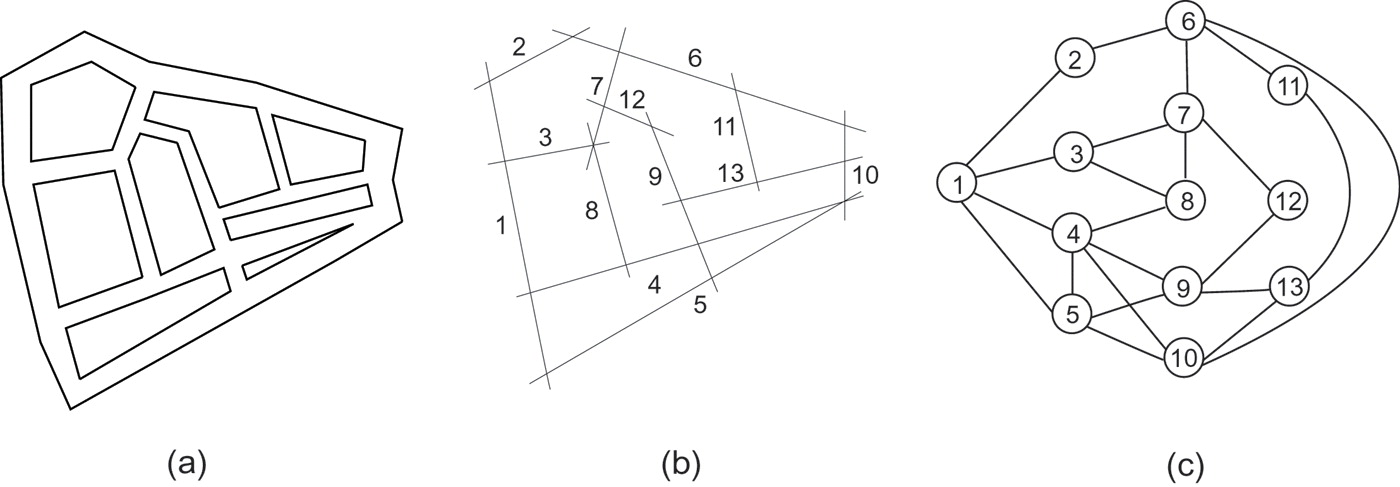
\includegraphics[width=\linewidth]{map_view.jpeg}
\caption{(a) A fictive urban system, (b) its axial map and (c) connectivity graph, taken from \cite{doi:10.1080/13658810802022822}}
\label{fig:city rep}
\end{figure}

This application is slightly different to the usual PR algorithm, as the graph formed from a urban space is a connected graph, and so there are no dangling nodes involved, in terms of a random walker, they will never get stuck, we assume that they never get tired and that they always move to one of its successors with non-uniform probability, as well-connected streets are preferable. Due to this non-uniform probability, we need to use the WPR algorithm as discussed in Section \ref{sec:weighted} as opposed to the standard algorithm.

\subsection{Durham} \label{sec:durham}
Jiang showed that PR scores are significantly correlated to human movement in four areas of London \cite{doi:10.1080/13658810802022822}, and we will use this methodology as a basis for our analysis of vehicle movement in Durham. 
\subsubsection{Methodology}
In order to represent the road network in Durham, we first produce an axial map and then are able to form a connectivity graph. The axial map is produced by taking a map of Durham, Figure \ref{fig:durham map}, and representing the intersections of the roads by a 'The axial map is constructed by taking an accurate map and drawing a set of intersecting lines through all the spaces of the urban grid so that the grid is covered and all rings of circulation are completed.' \cite{Axialmap40:online}, thus forming the axial map in Figure \ref{fig:durham axial}. This axial map can now be represented as a directed hypergraph, Figure \ref{fig:durham graph}. 

\begin{figure}[h]
\centering
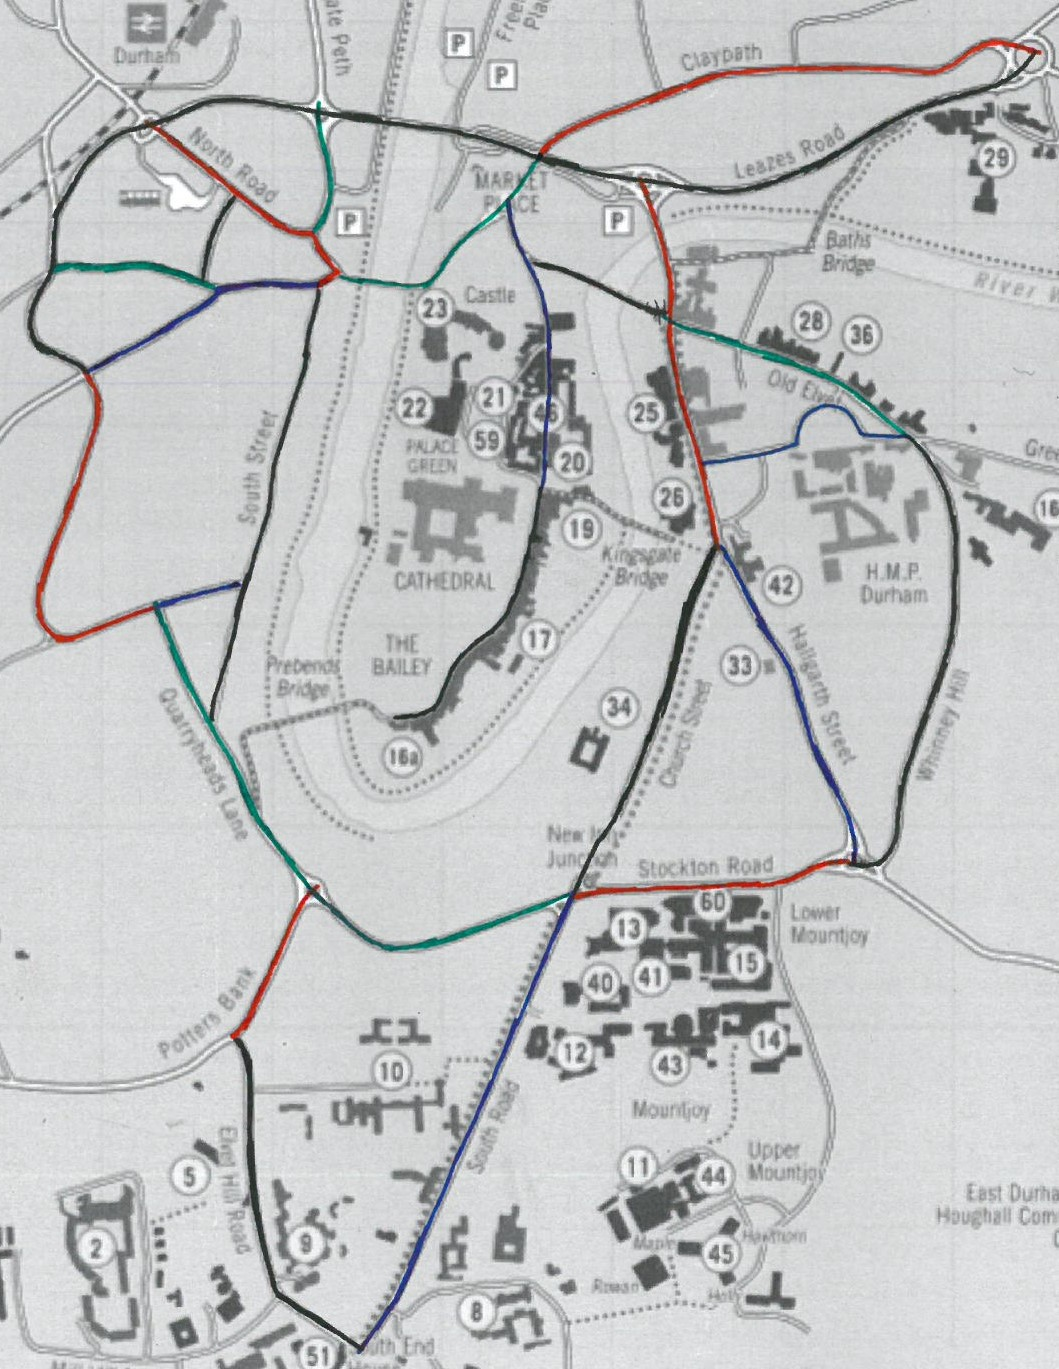
\includegraphics[width=\linewidth]{durham_with_colour.jpg}
\caption{Durham road network, adapted from \cite{undergraduate}}
\label{fig:durham map}
\end{figure}

\begin{figure}[h]
\centering
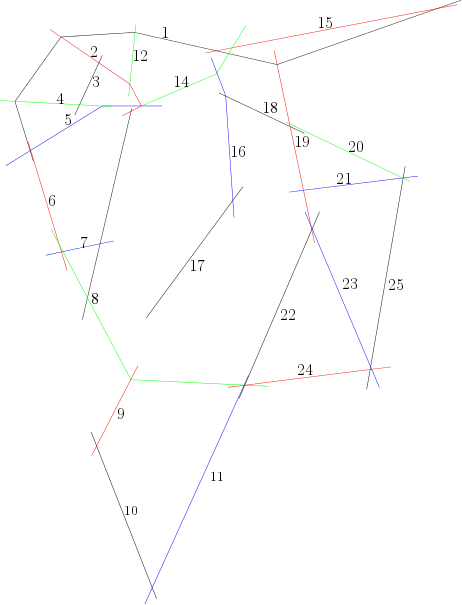
\includegraphics[width=10cm]{axial_colour_label.png}
\caption{Durham road network represented by an axial graph}
\label{fig:durham axial}
\end{figure}

\begin{figure}[h]
\centering
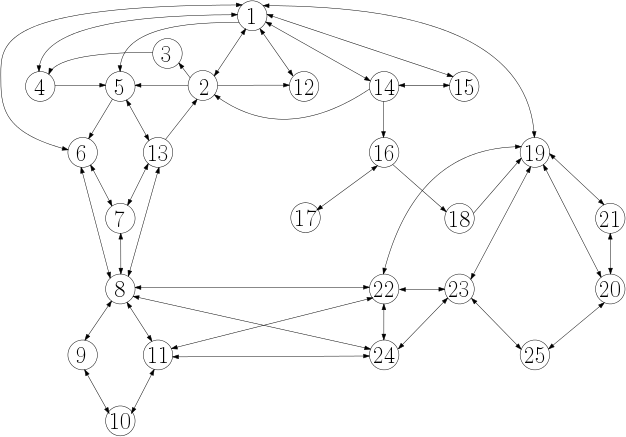
\includegraphics[width=10cm]{ipe_durham.png}
\caption{Durham road network represented by a hypergraph}
\label{fig:durham graph}
\end{figure}
\FloatBarrier


\subsubsection{Results and Analysis} \label{sec:results}

\begin{table}[h] \caption{Comparison of PageRankings produced by standard algorithm and the WPR algorithm on Durham}
 \centering
 \begin{tabular} {r l| c c} 
 \multicolumn{2}{c|}{Node}& PR & WPR \\ [0.5ex] 
 \hline
 1&A390&1&1\\
 2&North Rd&8&8\\
 3&Neville St&19&22\\
 4&Allergate&22&19\\
 5&Crossgate&24&24\\
 6&Margery Ln&6&11\\
 7&Grove St&23&23\\
 8&Quarryheads Ln&11&6\\
 9&Potters Bank&13&2\\
 10&Elvet Hill Rd&7&17\\
 11&South Rd&5&18\\
 12&Milburngate&20&25\\
 13&South St&25&13\\
 14&Silver St&2&14\\
 15&Claypath&9&4\\
 16&Saddler St&10&7\\
 17&Bailey&4&5\\
 18&Elvet Bridge&16&20\\
 19&New Elvet&14&5\\
 20&Old Elvet&12&9\\
 21&Court Ln&15&12\\
 22&Church St&21&10\\
 23&Stockton Rd&17&21\\
 24&Hallgarth St&18&16\\
 25&Whinney Hill&3&3\\
 
 \end{tabular}
 \label{Table:Durham comparison}
\end{table}
\FloatBarrier

\subsubsection{Conclusion} \label{sec:Durham conc}

%--------------------Conclusion
\chapter{Conclusion} \label{chap:Conclusion}
%--------------------Bibliography
\newpage
\addcontentsline{toc}{chapter}{Bibliography}

\bibliographystyle{plain}
\bibliography{bibliography.bib}
%--------------------Appendices

\begin{appendices}
\chapter{Google Matrix}
\begin{align*}
\textbf{G} &  = 0.85\cdot\textbf{H} + (0.85\cdot\textbf{a} + 0.15)\left(\frac{1}{n}\cdot 1^T\right)\\
& = 0.85\cdot\textbf{H} + \left((0.85\left(\begin{array}{c}
0\\0\\0\\0\\0\\0\\1\\0\end{array}\right) + 0.15\left(\begin{array}{c}
1\\1\\1\\1\\1\\1\\1\\1\end{array}\right)\right)\left(\frac{1}{8}\cdot\left(\begin{array}{cccccccc}
1&1&1&1&1&1&1&1\end{array}\right)\right)\\
&= 0.85\left(
\begin{array}{cccccccc}
0 & 0.28\overline{3} & 0 & 0.28\overline{3} & 0 & 0.28\overline{3} & 0 & 0  \\
0 & 0 & 0.425 & 0 & 0.425 & 0 & 0 & 0  \\
0 & 0 & 0 & 0 & 0.850 & 0 & 0 & 0  \\
0 & 0 & 0 & 0 & 0.425 & 0 & 0.425 & 0  \\
0 & 0 & 0 & 0 & 0 & 0 & 0 & 0.850  \\
0 & 0 & 0 & 0.28\overline{3} & 0 & 0 & 0.28\overline{3} & 0.28\overline{3}  \\
0 & 0 & 0 & 0 & 0 & 0 & 0 & 0  \\
0 & 0 & 0 & 0 & 0.425 & 0 & 0.425 & 0  \\
\end{array}
\right) \\&+ \left(
\begin{array}{cccccccc}
0.019 & 0.019 & 0.019 & 0.019 & 0.019 & 0.019 & 0.019 & 0.019  \\
0.019 & 0.019 & 0.019 & 0.019 & 0.019 & 0.019 & 0.019 & 0.019  \\
0.019 & 0.019 & 0.019 & 0.019 & 0.019 & 0.019 & 0.019 & 0.019  \\
0.019 & 0.019 & 0.019 & 0.019 & 0.019 & 0.019 & 0.019 & 0.019  \\
0.019 & 0.019 & 0.019 & 0.019 & 0.019 & 0.019 & 0.019 & 0.019  \\
0.019 & 0.019 & 0.019 & 0.019 & 0.019 & 0.019 & 0.019 & 0.019  \\
0.125 & 0.125 & 0.125 & 0.125 & 0.125 & 0.125 & 0.125 & 0.125  \\
0.019 & 0.019 & 0.019 & 0.019 & 0.019 & 0.019 & 0.019 & 0.019 
\end{array}
\right)\\
&= \left(
\begin{array}{cccccccc}
0.019 & 0.302 & 0.019 & 0.302 & 0.019 & 0.302 & 0.019 & 0.019  \\
0.019 & 0.019 & 0.444 & 0.019 & 0.444 & 0.019 & 0.019 & 0.019  \\
0.019 & 0.019 & 0.019 & 0.019 & 0.869 & 0.019 & 0.019 & 0.019  \\
0.019 & 0.019 & 0.019 & 0.019 & 0.444 & 0.019 & 0.444 & 0.019  \\
0.019 & 0.019 & 0.019 & 0.019 & 0.019 & 0.019 & 0.019 & 0.869  \\
0.019 & 0.019 & 0.019 & 0.302 & 0.019 & 0.019 & 0.302 & 0.302  \\
0.125 & 0.125 & 0.125 & 0.125 & 0.125 & 0.125 & 0.125 & 0.125  \\
0.019 & 0.019 & 0.019 & 0.019 & 0.444 & 0.019 & 0.444 & 0.019 
\end{array}
\right)
\end{align*} 
%--------------------
\chapter{Durham Results}
\begin{figure} [h!]  
\begin{equation*} \renewcommand*{\arraystretch}{1.05}
\left(
\begin{array}{ccccccccccccccccccccccccc}
0&\frac{1}{8}&0&\frac{1}{8}&\frac{1}{8}&\frac{1}{8}&0&0&0&0&0&\frac{1}{8}&0&\frac{1}{8}&\frac{1}{8}&0&0&0&\frac{1}{8}&0&0&0&0&0&0\\

\frac{1}{4}&0&\frac{1}{4}&0&\frac{1}{4}&0&0&0&0&0&0&\frac{1}{4}&0&0&0&0&0&0&0&0&0&0&0&0&0\\

0&0&0&1&0&0&0&0&0&0&0&0&0&0&0&0&0&0&0&0&0&0&0&0&0\\

\frac{1}{2}&0&0&0&\frac{1}{2}&0&0&0&0&0&0&0&0&0&0&0&0&0&0&0&0&0&0&0&0\\

0&0&0&0&0&\frac{1}{2}&0&0&0&0&0&0&\frac{1}{2}&0&0&0&0&0&0&0&0&0&0&0&0\\

\frac{1}{3}&0&0&0&0&0&\frac{1}{3}&\frac{1}{3}&0&0&0&0&0&0&0&0&0&0&0&0&0&0&0&0&0\\

0&0&0&0&0&\frac{1}{3}&0&\frac{1}{3}&0&0&0&0&\frac{1}{3}&0&0&0&0&0&0&0&0&0&0&0&0\\

0&0&0&0&0&\frac{1}{7}&\frac{1}{7}&0&\frac{1}{7}&0&\frac{1}{7}&0&\frac{1}{7}&0&0&0&0&0&0&0&0&\frac{1}{7}&0&\frac{1}{7}&0\\

0&0&0&0&0&0&0&\frac{1}{2}&0&\frac{1}{2}&0&0&0&0&0&0&0&0&0&0&0&0&0&0&0\\

0&0&0&0&0&0&0&0&\frac{1}{2}&0&\frac{1}{2}&0&0&0&0&0&0&0&0&0&0&0&0&0&0\\

0&0&0&0&0&0&0&\frac{1}{4}&0&\frac{1}{4}&0&0&0&0&0&0&0&0&0&0&0&\frac{1}{4}&0&\frac{1}{4}&0\\

1&0&0&0&0&0&0&0&0&0&0&0&0&0&0&0&0&0&0&0&0&0&0&0&0\\

0&\frac{1}{4}&0&0&\frac{1}{4}&0&\frac{1}{4}&\frac{1}{4}&0&0&0&0&0&0&0&0&0&0&0&0&0&0&0&0&0\\

\frac{1}{4}&\frac{1}{4}&0&0&0&0&0&0&0&0&0&0&0&0&\frac{1}{4}&\frac{1}{4}&0&0&0&0&0&0&0&0&0\\

\frac{1}{2}&0&0&0&0&0&0&0&0&0&0&0&0&\frac{1}{2}&0&0&0&0&0&0&0&0&0&0&0\\

0&0&0&0&0&0&0&0&0&0&0&0&0&0&0&0&\frac{1}{2}&\frac{1}{2}&0&0&0&0&0&0&0\\

0&0&0&0&0&0&0&0&0&0&0&0&0&0&0&1&0&0&0&0&0&0&0&0&0\\

0&0&0&0&0&0&0&0&0&0&0&0&0&0&0&0&0&0&1&0&0&0&0&0&0\\

\frac{1}{4}&0&0&0&0&0&0&0&0&0&0&0&0&0&0&0&0&0&0&\frac{1}{4}&0&\frac{1}{4}&\frac{1}{4}&0&0\\

0&0&0&0&0&0&0&0&0&0&0&0&0&0&0&0&0&0&\frac{1}{3}&0&\frac{1}{3}&0&0&0&\frac{1}{3}\\

0&0&0&0&0&0&0&0&0&0&0&0&0&0&0&0&0&0&\frac{1}{2}&\frac{1}{2}&0&0&0&0&0\\

0&0&0&0&0&0&0&\frac{1}{5}&0&0&\frac{1}{5}&0&0&0&0&0&0&0&\frac{1}{5}&0&0&0&\frac{1}{5}&\frac{1}{5}&0\\

0&0&0&0&0&0&0&0&0&0&0&0&0&0&0&0&0&0&\frac{1}{4}&0&0&\frac{1}{4}&0&\frac{1}{4}&\frac{1}{4}\\

0&0&0&0&0&0&0&\frac{1}{5}&0&0&\frac{1}{5}&0&0&0&0&0&0&0&0&0&0&\frac{1}{5}&\frac{1}{5}&0&\frac{1}{5}\\

0&0&0&0&0&0&0&0&0&0&0&0&0&0&0&0&0&0&0&\frac{1}{3}&0&0&\frac{1}{3}&\frac{1}{3}&0\\

\end{array}
\right)
\end{equation*} 
\caption{Hyperlink matrix for Durham}
\end{figure}  \label{fig:DH}

\begin{landscape}
\begin{figure} [h!] 
\begin{equation*} \renewcommand*{\arraystretch}{1.25}
\left(
\begin{array}{ccccccccccccccccccccccccc}
\frac{53}{92}&\frac{1}{42}&\frac{1}{84}&\frac{1}{42}&\frac{1}{53}&0&\frac{2}{63}&\frac{2}{27}&0&0&0&\frac{1}{84}&0&\frac{2}{63}&\frac{1}{84}&\frac{1}{84}&0&0&0&\frac{3}{70}&0&\frac{1}{14}&\frac{2}{35}&0&0\\

\frac{1}{12}&\frac{4}{19}&0&\frac{1}{19}&\frac{8}{95}&\frac{7}{88}&\frac{3}{64}&\frac{7}{64}&0&0&0&\frac{1}{38}&0&\frac{7}{66}&\frac{2}{27}&\frac{1}{48}&0&0&\frac{7}{66}&0&0&0&0&0&0\\

0&0&0&1&0&0&0&0&0&0&0&0&0&0&0&0&0&0&0&0&0&0&0&0&0\\

0&\frac{7}{44}&0&\frac{9}{44}&\frac{7}{88}&0&\frac{8}{67}&0&0&0&0&\frac{1}{25}&0&\frac{7}{44}&\frac{7}{88}&0&0&0&\frac{7}{44}&0&0&0&0&0&0\\

\frac{6}{25}&\frac{12}{89}&\frac{1}{60}&\frac{5}{66}&\frac{8}{85}&\frac{3}{47}&\frac{3}{80}&\frac{7}{80}&0&0&0&\frac{3}{79}&0&\frac{4}{47}&\frac{2}{47}&0&0&0&\frac{4}{47}&0&0&0&0&0&0\\

0&\frac{2}{33}&0&\frac{1}{33}&\frac{1}{33}&\frac{19}{97}&\frac{1}{26}&\frac{1}{14}&\frac{1}{39}&0&\frac{2}{39}&\frac{1}{66}&\frac{1}{5}&\frac{2}{33}&\frac{1}{33}&0&0&0&\frac{2}{33}&0&0&\frac{5}{78}&0&\frac{5}{78}&0\\

\frac{8}{63}&\frac{3}{56}&0&0&\frac{2}{75}&\frac{3}{52}&\frac{8}{55}&\frac{17}{83}&\frac{1}{26}&0&\frac{1}{13}&0&\frac{1}{13}&0&0&0&0&0&0&0&0&\frac{5}{52}&0&\frac{5}{52}&0\\

\frac{5}{73}&\frac{1}{35}&0&0&\frac{1}{70}&\frac{2}{81}&\frac{1}{21}&\frac{21}{52}&0&\frac{1}{30}&\frac{3}{44}&0&\frac{2}{61}&0&0&0&0&0&\frac{3}{86}&0&0&\frac{6}{73}&\frac{3}{44}&\frac{3}{74}&\frac{2}{39}\\

0&0&0&0&0&\frac{7}{78}&\frac{7}{78}&0&\frac{2}{15}&0&\frac{19}{71}&0&\frac{3}{25}&0&0&0&0&0&0&0&0&\frac{3}{20}&0&\frac{3}{20}&0\\

0&0&0&0&0&0&0&\frac{1}{2}&0&\frac{1}{7}&0&0&0&0&0&0&0&0&0&0&0&\frac{10}{57}&0&\frac{10}{57}&0\\

0&0&0&0&0&\frac{2}{47}&\frac{2}{47}&\frac{9}{55}&\frac{5}{79}&0&\frac{11}{50}&0&\frac{3}{53}&0&0&0&0&0&\frac{1}{21}&0&0&\frac{11}{86}&\frac{3}{32}&\frac{7}{99}&\frac{4}{57}\\

\frac{1}{5}&\frac{7}{55}&\frac{1}{40}&\frac{5}{44}&\frac{4}{63}&\frac{2}{21}&0&0&0&0&0&\frac{5}{88}&0&\frac{7}{55}&\frac{4}{63}&0&0&0&\frac{7}{55}&0&0&0&0&0&0\\

0&0&0&0&0&\frac{19}{84}&\frac{3}{52}&\frac{3}{28}&\frac{1}{26}&0&\frac{1}{13}&0&\frac{19}{63}&0&0&0&0&0&0&0&0&\frac{5}{52}&0&\frac{5}{52}&0\\

\frac{4}{27}&\frac{14}{99}&0&\frac{7}{99}&\frac{7}{99}&\frac{7}{55}&0&0&0&0&0&\frac{3}{85}&0&\frac{14}{65}&\frac{7}{99}&0&0&0&\frac{14}{99}&0&0&0&0&0&0\\

\frac{1}{9}&\frac{13}{66}&0&\frac{7}{99}&\frac{7}{99}&\frac{7}{55}&0&0&0&0&0&\frac{3}{85}&0&\frac{14}{99}&\frac{6}{61}&\frac{1}{36}&0&0&\frac{14}{99}&0&0&0&0&0&0\\

\frac{1}{2}&\frac{1}{4}&0&0&0&0&0&0&0&0&0&0&0&0&\frac{1}{8}&\frac{1}{8}&0&0&0&0&0&0&0&0&0\\

0&0&0&0&0&0&0&0&0&0&0&0&0&0&0&0&\frac{1}{2}&\frac{1}{2}&0&0&0&0&0&0&0\\

0&0&0&0&0&0&0&0&0&0&0&0&0&0&0&0&\frac{1}{2}&\frac{1}{2}&0&0&0&0&0&0&0\\

0&\frac{2}{33}&0&\frac{1}{33}&\frac{1}{33}&\frac{1}{22}&0&\frac{5}{66}&0&0&\frac{1}{23}&\frac{1}{66}&0&\frac{2}{33}&\frac{1}{33}&0&0&0&\frac{23}{80}&\frac{2}{97}&\frac{2}{63}&\frac{1}{18}&\frac{1}{23}&\frac{1}{18}&\frac{5}{44}\\

\frac{6}{25}&0&0&0&0&0&0&0&0&0&0&0&0&0&0&0&0&0&\frac{2}{35}&\frac{16}{77}&0&\frac{3}{20}&\frac{11}{50}&\frac{1}{8}&0\\

0&0&0&0&0&0&0&0&0&0&0&0&0&0&0&0&0&0&\frac{4}{9}&0&\frac{2}{9}&0&0&0&\frac{1}{3}\\

\frac{6}{65}&0&0&0&0&\frac{1}{32}&\frac{1}{32}&\frac{3}{26}&\frac{1}{48}&\frac{1}{62}&\frac{3}{40}&0&\frac{1}{24}&0&0&0&0&0&\frac{2}{55}&\frac{1}{29}&0&\frac{23}{97}&\frac{7}{88}&\frac{11}{80}&\frac{1}{19}\\

\frac{11}{87}&0&0&0&0&0&0&\frac{9}{55}&0&0&\frac{3}{32}&0&0&0&0&0&0&0&\frac{1}{21}&\frac{2}{23}&0&\frac{3}{22}&\frac{9}{43}&\frac{5}{76}&\frac{4}{57}\\

0&0&0&0&0&\frac{2}{57}&\frac{2}{57}&\frac{2}{15}&\frac{1}{43}&\frac{1}{55}&\frac{5}{58}&0&\frac{3}{64}&0&0&0&0&0&\frac{7}{87}&\frac{1}{31}&0&\frac{7}{45}&\frac{1}{12}&\frac{13}{62}&\frac{5}{83}\\

0&0&0&0&0&0&0&\frac{8}{63}&0&0&\frac{5}{69}&0&0&0&0&0&0&0&\frac{18}{95}&0&\frac{1}{18}&\frac{10}{53}&\frac{5}{69}&\frac{5}{51}&\frac{11}{56}\\

\end{array}
\right)
\end{equation*} 
\caption{Weighted hyperlink matrix for Durham}
\end{figure}  \label{fig:DWH}
\end{landscape}

\begin{figure} [H]  
\begin{equation} 
\boldsymbol\pi_{PR} = \left(
\begin{array}{c}
0.0857\\
0.0300\\
0.0124\\
0.0256\\
0.0423\\
0.0557\\
0.0423\\
0.0867\\
0.0289\\
0.0289\\
0.0499\\
0.0215\\
0.0466\\
0.0237\\
0.0201\\
0.0252\\
0.0167\\
0.0167\\
0.0696\\
0.0389\\
0.0107\\
0.0634\\
0.0527\\
0.0601\\
0.0384
\end{array}
\right) \qquad 
\boldsymbol\pi_{WPR} = \left(
\begin{array}{c}
0.1023 \\
0.0443 \\
0.0077 \\
0.0313 \\
0.0240 \\
0.0482 \\
0.0295 \\
0.1090 \\
0.0163 \\
0.0126 \\
0.0497 \\
0.0137 \\
0.0379 \\
0.0353 \\
0.0215 \\
0.0093 \\
0.0400 \\
0.0400 \\
0.0691 \\
0.0223 \\
0.0120 \\
0.0785 \\
0.0482 \\
0.0555 \\
0.0396 
\end{array}
\right)
\end{equation} 
\caption{PR and WPR vectors for Durham}
\end{figure}  \label{fig:DPR}
\begin{table}[h] \caption{Number of cars at each node}
\centering
 \begin{tabular} {r l| c } 
 \multicolumn{2}{c|}{Node} & Cars \\ [0.5ex] 
 \hline
 \multirow{6}{*}{1}&\multirow{6}{*}{A390}&\\
 & &\\ 
 & &\\
 & &\\
 & &\\
 & &\\
  \hline
\multirow{3}{*}{2}& \multirow{3}{*}{North Rd}&\\
  &&\\
  &&\\
  \hline
 3&Neville St&\\
  \hline
 4&Allergate&\\
  \hline
\multirow{2}{*}{5}&\multirow{2}{*}{Crossgate}&\\
& &\\ 
 \hline
 6 &Margery Ln&\\
 \hline
 7 & Grove St&\\
 \hline
 \multirow{3}{*}{8}&\multirow{3}{*}{Quarryheads Ln}&\\
 &&\\
 &&\\
 \hline
 9 & Potters Bank&\\
 \hline
 10 & Elvet Hill Rd&\\
 \hline
 11 & South Rd&\\
 \hline
 12 & Milburngate&\\
 \hline
 \multirow{2}{*}{13}&\multirow{2}{*}{South St}&\\
 &&\\  
 \hline
 \multirow{2}{*}{14}&\multirow{2}{*}{Silver St}&\\
 &&\\
 \hline
 15& Claypath&\\
 \hline
 \multirow{2}{*}{16}&\multirow{2}{*}{Saddler St}&\\
 &&\\
 \hline
 17& Bailey&\\
 \hline
 18 & Elvet Bridge&\\
 \hline
 \multirow{3}{*}{19}&\multirow{3}{*}{New Elvet}&\\
 &&\\
 &&\\
 \hline
 20 & Old Elvet&\\
 \hline
 21 & Court Ln&\\
 \hline
 22 & Church St&\\
 \hline
 23 &Stockton Rd&\\
 \hline
 24 & Hallgarth St&\\
 \hline
 25 & Whinney Hill&\\ 
 
 \end{tabular}
 \label{Table:Durham cars}
\end{table}

\chapter{Matlab code} \label{app:code}

\begin{lstlisting} [caption=Matlab code for implementing power method taken from \cite{langville} ]
function [pi,time,numiter] = \hbox{PageRank}(pi0,H,n,alpha,epsilon);

% \hbox{PageRank} computes the \hbox{PageRank} vector for an n-by-n Markov
%           matrix H with starting vector pi0 (a row vector)
%           and scaling parameter alpha (scalar). Uses power method.
%
% EXAMPLE: [pi,time,numiter] = \hbox{PageRank}(pi0,H,1000,.9,1e-8)
%
% INPUT: pi0 = starting vector at iteration 0 (row vector)
%        H = row-normalized hyperlink matrix (n-by-n sparse matrix)
%        n = size of H matrix (scalar)
%        alpha = scaling parameter in \hbox{PageRank} model (scalar)
%        epsilon = convergence tolerance (scalar, e.g. 1e-8)
%
% OUTPUT: pi = \hbox{PageRank} vector
%         time = time required to compute \hbox{PageRank} vector
%         numiter = number of iterations until convergence
%        
% Starting vector is usually set to uniform vector,
% pi0=1/n*ones(1,n).
% NOTE: Matlab stores sparse matrices by columns, so it is faster
%       to do some operations on H', the transpose of H.
% get 'a', dangling node vector, where a(i) = 1, if node i 
%    is dangling node and 0 o.w.

rowsumvector = ones(1,n)*H';
nonzerorows=find(rowsumvector);
zerorows=setdiff(1:n,nonzerorows); l=length(zerorows);
a=sparse(zerorows,ones(1,1),ones(1,1),n,1);

k=0;
residual=1;
pi=pi0;
tic;

while(residual>=epsilon)
     prevpi=pi;
     k=k+1;
     pi=alpha*pi*H + (alpha*(pi*a)+1-alpha)*((1/n)*ones(1,n));
     residual=norm(pi-prevpi,1);
end

numiter=k;
time=toc;

\end{lstlisting}

\begin{lstlisting} [caption=Matlab code for implementing HITS power method taken from \cite{langville}]
function [x,y,time,numiter] = hits[L,x0,n,epsilon] 

% HITS computes the HITS authority vector x and hub vector y 
%      for an n-by-n adjacency matrix L with starting vector
%      x0 (a row vector). Uses power method on L'*L.
%
% EXAMPLE: [x,y,time,numiter] = hits[L,x0,100,1e-8]
%
% INPUT: L = adjacency matrix (n-by-n sparse matrix)
%        x0 = starting vector (row vector)
%        n = size of L matrix (integer)
%        epsilon = convergence tolerance (scalar, e.g. 1e-8)
%
% OUTPUT: x = HITS authority vector
%         y = HITS hub vector
%         time = time until convergence
%         numiter = number of iterations until convergence
%        
% The starting vector is usually set to the uniform vector,
% x0=1/n*ones(1/n)

k=0;
residual=1;
x=x0;
tic;

while(residual>=epsilon)
     prevx=x;
     k=k+1;
     x=x*L';
     x=x*L;
     x=x/sum(x);
     residual=norm(x-prevx,1);
end
y=x*L';
y=y/sum(y);
numiter=k;
time=toc;

\end{lstlisting}
\end{appendices}




\end{document}